% !TeX program = pdflatex
% !TeX spellcheck = en_US
% !TeX encoding = UTF-8

\documentclass[twoside,11pt,titlepage,a4paper,english,bibliography=totocnumbered,listof=numbered]{scrbook}
%
% Template Style
% =========================================================================
% = SNET THESIS TEMPLATE STYLE
% =========================================================================

% http://www.snet.tu-berlin.de
% ------------------------
% Adapted version from http://hci.rwth-aachen.de/karrer_thesistemplate (Thorsten Karrer)
% Further adaptions for http://www.elearn.rwth-aachen.de (Sascha Hoellger)
% Further adaptions for SNET @ TU Berlin by Sebastian Göndör (sebastian.goendoer@tu-berlin.de)


% =========================================================================
% = CHANGELOG
% =========================================================================
% [0.1.9]
% - Fixed styling for chapters and toc using Komascript
% - Remove double bibliography TOC entry
%
% [0.1.8]
% - fixed "warning UFT8 is used". biblatex requires ascii encoding; by Dirk
%
% [0.1.7]
% replaced "Titelsec" commands (and whole package) by appropriate KOMA-Script commands; by Dirk
%
% [0.1.6]
% replaced deprecated \rm commands with \rmfamily commands; by Dirk
%
% [0.1.4b]
% backend=biber added in line 139
%
% [0.1.4a]
% title page: image logo sizes and margins adjusted to printable area
% removed separation of online and offline references
%
% [0.1.3]
% wider text body
% added "school" to the titlepage
% paragraph indents
% correctly placed footnote graphics
%
% [0.1.2]
% new titlepage
% some minor fixes
%
% [0.1.1]
% changed titlepage logo
% added listoffigures and listoftables
% excluded abstract from toc
% no (roman) numbering for frontmatter
%
% [0.1]
% adapted version 0.991b from sascha hoellger @ rwth aachen


% =========================================================================
% = MISC
% =========================================================================

\usepackage{a4wide}					%
\usepackage{verbatim}				%
\usepackage[toc,page]{appendix}			%
\usepackage[withpage]{acronym}			%
\usepackage{amsthm}				% Definitions


% =========================================================================
% = COLORS
% =========================================================================

\usepackage{xcolor}					% Colors
\definecolor{LightBlue}{rgb}{0.55,0.55,1}
\definecolor{DarkBlue}{rgb}{0.2,0.2,0.5}
\definecolor{DarkRed}{rgb}{0.7725490196,0.05490196078,0.12549019607} % new TU red
\definecolor{Black}{rgb}{0,0,0}

% =========================================================================
% = PAGE LAYOUT
% =========================================================================

\usepackage{geometry}
\geometry{inner=3cm, outer=2cm, bottom=4cm}

\newcommand{\setwidesite}				% changes the geometry to have less margin
{
	\fancyhfoffset[LE,RO]{0cm}
	\fancyheadoffset[LO,RE]{0cm}
	\fancyfootoffset[RE]{2cm}
	\newgeometry{inner=2cm, outer=2cm, bottom=4cm}
}

\usepackage{style/noindent}				%do not indent at new paragraphs but add a vertical offset

\setlength{\parindent}{4mm}
\setlength{\parskip}{1.5mm }


% =========================================================================
% = TYPESETTING
% =========================================================================

\usepackage[hyphens]{url}				% url
\usepackage{hyphenat}				% hyphenation. use \hyphenation{}

\righthyphenmin=5
\lefthyphenmin=5


% =========================================================================
% = TABLE OF CONTENTS
% =========================================================================

\setcounter{secnumdepth}{4}
\setcounter{tocdepth}{3}

\addtokomafont{disposition}{\rmfamily}


% =========================================================================
% = FONTS
% =========================================================================

\usepackage{mathpazo}
\usepackage[scaled=.95]{helvet}
\usepackage{courier}


% =========================================================================
% = SYMBOLS
% =========================================================================

%\usepackage{gensymb}
\usepackage{textcomp} 				% for \textmu (non-italic $\mu$)
\makeatletter						% this makes "@" a regular letter


% =========================================================================
% = TABLES
% =========================================================================

\usepackage{tabularx}
\usepackage{booktabs}
\usepackage{multirow}
\usepackage{longtable}				% tables spanning over more than one page

%%\setlength{\fboxsep}{0mm}			% spacing between \fbox border and content

\usepackage{amsmath}				% math fonts
\usepackage{amssymb}				% math symbols
\usepackage{setspace}				% line spacing


% =========================================================================
% = BIBILOGRAPHY
% =========================================================================

% 2018-10-16 - changed to use Bibtex instead

%\usepackage[style=numeric,natbib=true,backend=biber]{biblatex}

% apparently no effect?
%\renewcommand{\bibsetup}{
%	\markboth{
%		\MakeUppercase{Bibliography}
%	}{}
%}

%\ifdefined\bibheadingonline
%  \defbibheading{online}{\section*{\bibheadingonline}}
%\else
%  \defbibheading{online}{\section*{Online References}}
%\fi
%\ifdefined\bibheadingoffline
%  \defbibheading{offline}{\section*{\bibheadingoffline}}
%\else
%  \defbibheading{offline}{\section*{Printed References}}
%\fi
%
%\defbibfilter{online}{%
%  \( \type{online} \)}
%
%\defbibfilter{offline}{%
%  \( \not \type{online} \)}
%
%\bibliography{Bibliography}


% =========================================================================
% = LANGUAGE & ENCODING
% =========================================================================

\usepackage[english]{babel}				% \usepackage[ngerman]{babel}

\selectlanguage{english}				% \selectlanguage{ngerman}

\usepackage[T1]{fontenc}
\usepackage[utf8]{inputenc}				% can use native umlauts

% \usepackage[babel,german=quotes]{csquotes}	% provides \enquote{Blupp} => "`Blupp"'
\usepackage[babel,english=american]{csquotes}	% provides \enquote{Blupp} => "`Blupp"'

%\SetCiteCommand{\parencite}			% Changed for biblatex

\usepackage{units}					% unified way of setting values with units

\usepackage{appendix}


% =========================================================================
% = CODE LISTINGS
% =========================================================================

\usepackage{listings}

% Listings Styles from Max

\definecolor{violet}{cmyk}{0.45,0.97,0.27,0.21}
\definecolor{lstblue}{cmyk}{1,0.80,0,0}
\definecolor{lstgreen}{cmyk}{0.71,0.21,0.65,0.22}
\definecolor{bluegrey}{cmyk}{0.56,0.24,0.11,0.05}
\definecolor{javadoc}{cmyk}{0.88,0.59,0,0}
\definecolor{lstgrey}{cmyk}{0.55,0.44,0.42,0.32}

\lstdefinelanguage{SQL}{
     keywords={},
     keywordstyle=\color{bluegrey}\bfseries,
     morekeywords=[2]{CREATE,TABLE,IF,NOT,EXISTS,NULL,SET,DEFAULT,PRIMARY,KEY,COLLATE,CHARACTER,AUTO_INCREMENT,ENGINE,CHARSET},
     keywordstyle={[2]\color{violet}\bfseries},
     otherkeywords={int,varchar,double,text,tinyint},
     sensitive=false,
     morecomment=[l][\color{lstgreen}]{//},
     morecomment=[s][\color{lstgreen}]{/*}{*/},
     morecomment=[s][\color{javadoc}]{/**}{*/},
     morestring=[b]',
     morestring=[b]"
  }
\lstdefinelanguage{PHP}{
     keywords={},
     keywordstyle=\color{bluegrey}\bfseries,
     morekeywords=[2]{static,function,if,return,pow,sin,cos,asin,min,sqrt,int},
     keywordstyle={[2]\color{violet}\bfseries},
     otherkeywords={@param, @returns, @author, @type, @link, @see},
     sensitive=false,
     morecomment=[l][\color{lstgreen}]{//},
     morecomment=[s][\color{lstgreen}]{/*}{*/},
     morecomment=[s][\color{javadoc}]{/**}{*/},
     morestring=[b]',
     morestring=[b]"
  }
\lstdefinelanguage{JavaScript}{
     keywords={},
     keywordstyle=\color{bluegrey}\bfseries,
     morekeywords=[2]{attributes, class, classend, do, empty, endif, endwhile, fail, function, functionend, if, implements, in, inherit, inout, not, of, operations, out, return, set, then, types, while, use},
     keywordstyle={[2]\color{violet}\bfseries},
     otherkeywords={@param, @returns, @author, @type, @link, @see},
     sensitive=false,
     morecomment=[l][\color{lstgreen}]{//},
     morecomment=[s][\color{lstgreen}]{/*}{*/},
     morecomment=[s][\color{javadoc}]{/**}{*/},
     morestring=[b]',
     morestring=[b]"
  }
\lstdefinelanguage{Java}{
     keywords={},
     keywordstyle=\color{bluegrey}\bfseries,
     morekeywords=[2]{abstract,boolean,break,byte,case,catch,char,class,
      const,continue,default,do,double,else,extends,false,final,
      finally,float,for,goto,if,implements,import,instanceof,int,
      interface,label,long,native,new,null,package,private,protected,
      public,return,short,static,super,switch,synchronized,this,throw,
      throws,transient,true,try,void,volatile,while},
     keywordstyle={[2]\color{violet}\bfseries},
     morekeywords=[3]{@SuppressWarnings, @Capability, @Override},
     keywordstyle={[3]\color{lstgrey}},
     otherkeywords={@param, @return, @returns, @author, @link, @see},
     sensitive,
     morecomment=[l]//,
     morecomment=[s]{/*}{*/},
     morecomment=[s][\color{javadoc}]{/**}{*/},
     morestring=[b]",
     morestring=[b]',
  }[keywords,comments,strings]

% some listings styles from Gregor Aisch
% http://vis4.net/blog/2009/09/noch-mehr-sprach-definitionen-fuer-latex-listings/

\lstdefinelanguage{HTML5} {morekeywords={a, abbr, address, area, article, aside, audio, b, base, bb, bdo, blockquote,  body, br, button, canvas, caption, cite, code, col, colgroup, command, datagrid, datalist, dd, del, details, dialog, dfn, div, dl, dt, em, embed, eventsource, fieldset, figure, footer,  form,  h1, h2,  h3,  h4, h5,  h6,  head,  header,  hr, html,  i, iframe,  img,  input,  ins, kbd,  label,  legend,  li,  link,  mark,  map,  menu,  meta,  meter,  nav,  noscript,  object,  ol,  optgroup,  option,  output,  p,  param,  pre,  progress,  q,  ruby,  rp,  rt,  samp,  script,  section,  select,  small,  source,  span,  strong,  style,  sub,  sup,  table,  tbody,  td,  textarea,  tfoot,  th,  thead,  time,  title,  tr,  ul,  var,  video},
sensitive=false, morecomment=[s]{<!--}{-->}, morestring=[b]", morestring=[d]'}

\lstdefinelanguage{CSS} {morekeywords={azimuth,  background-attachment,  background-color,  background-image,  background-position,  background-repeat,  background,  border-collapse,  border-color,  border-spacing,  border-style,  border-top, border-right, border-bottom, border-left,  border-top-color, border-right-color, border-bottom-color, border-left-color,  border-top-style, border-right-style, border-bottom-style, border-left-style,  border-top-width, border-right-width, border-bottom-width, border-left-width,  border-width,  border,  bottom,  caption-side,  clear,  clip,  color,  content,  counter-increment,  counter-reset,  cue-after,  cue-before,  cue,  cursor,  direction,  display,  elevation,  empty-cells,  float,  font-family,  font-size,  font-style,  font-variant,  font-weight,  font,  height,  left,  letter-spacing,  line-height,  list-style-image,  list-style-position,  list-style-type,  list-style,  margin-right, margin-left,  margin-top, margin-bottom,  margin,  max-height,  max-width,  min-height,  min-width,  orphans,  outline-color,  outline-style,  outline-width,  outline,  overflow,  padding-top, padding-right, padding-bottom, padding-left,  padding,  page-break-after,  page-break-before,  page-break-inside,  pause-after,  pause-before,  pause,  pitch-range,  pitch,  play-during,  position,  quotes,  richness,  right,  speak-header,  speak-numeral,  speak-punctuation,  speak,  speech-rate,  stress,  table-layout,  text-align,  text-decoration,  text-indent,  text-transform,  top,  unicode-bidi,  vertical-align,  visibility,  voice-family,  volume,  white-space,  widows,  width,  word-spacing,  z-index},
sensitive=false, morecomment=[s]{/*}{*/}, morestring=[b]", morestring=[d]'}

\lstdefinelanguage{JavaFX} {morekeywords={abstract, after, and, as, assert, at, attribute, before, bind, bound, break, catch, class, continue, def, delete, else, exclusive, extends, false, finally, first, for, from, function, if, import, indexof, in, init, insert, instanceof, into, inverse, last, lazy, mixin, mod, new, not, null, on, or, override, package, postinit, private, protected, public-init, public, public-read, replace, return, reverse, sizeof, static, step, super, then, this, throw, trigger, true, try, tween, typeof, var, where, while, with },
sensitive=false, morecomment=[l]{//}, morecomment=[s]{/*}{*/}, morestring=[b]", morestring=[d]'}

\lstdefinelanguage{MXML} {morekeywords={mx:Accordion, mx:Box, mx:Canvas, mx:ControlBar, mx:DividedBox, mx:Form, mx:FormHeading, mx:FormItem, mx:Grid, mx:GridItem, mx:GridRow, mx:HBox, mx:HDividedBox, mx:LinkBar, mx:Panel, mx:TabBar, mx:TabNavigator, mx:Tile, mx:TitleWindow, mx:VBox, mx:VDividedBox, mx:ViewStack, mx:Button, mx:CheckBox, mx:ComboBase, mx:ComboBox, mx:DataGrid, mx:DateChooser, mx:DateField, mx:HRule, mx:Image, mx:Label, mx:Link, mx:List, mx:Loader, mx:MediaController, mx:MediaDisplay, mx:MediaPlayback, mx:MenuBar, mx:NumericStepper, mx:ProgressBar, mx:RadioButton, mx:RadioButtonGroup, mx:Spacer, mx:Text, mx:TextArea, mx:TextInput, mx:Tree, mx:VRule, mx:VScrollBar, mx:Application, mx:Repeater, mx:UIComponent, mx:UIObject, mx:View, mx:FlexExtension, mx:UIComponentExtension, mx:UIObjectExtension, mx:Fade, mx:Move, mx:Parallel, mx:Pause, mx:Resize, mx:Sequence, mx:WipeDown, mx:WipeLeft, mx:WipeRight, mx:WipeUp, mx:Zoom, mx:EventDispatcher, mx:LowLevelEvents, mx:UIEventDispatcher, mx:CurrencyFormatter, mx:DateFormatter, mx:NumberFormatter, mx:PhoneFormatter, mx:ZipCodeFormatter, mx:CursorManager, mx:DepthManager, mx:DragManager, mx:FocusManager, mx:HistoryManager, mx:LayoutManager, mx:OverlappedWindows, mx:PopUpManager, mx:SystemManager, mx:TooltipManager, mx:CreditCardValidator, mx:DateValidator, mx:EmailValidator, mx:NumberValidator, mx:PhoneNumberValidator, mx:SocialSecurityValidator, mx:StringValidator, mx:ZipCodeValidator, mx:DownloadProgressBar, mx:ArrayUtil, mx:ClassUtil, mx:Delegate, mx:ObjectCopy, mx:URLUtil, mx:XMLUtil, mx:CSSSetStyle, mx:CSSStyleDeclaration, mx:CSSTextStyles, mx:StyleManager, mx:HTTPService, mx:RemoteObject, mx:Service},
sensitive=false, morecomment=[s]{<!--}{-->}, morestring=[b]", morestring=[d]'}

\lstdefinelanguage{LZX} {morekeywords={a, alert, animator, animatorgroup , attribute, audio , axis, axisstyle , b, barchart, basebutton , basebuttonrepeater , basecombobox , basecomponent , basedatacombobox , basedatepicker , basedatepickerday , basedatepickerweek , basefloatinglist , basefocusview , baseform , baseformitem , basegrid , basegridcolumn , baselist , baselistitem , basescrollarrow , basescrollbar , basescrollthumb , basescrolltrack , baseslider , basestyle , basetab , basetabelement , basetabpane , basetabs , basetabsbar , basetabscontent , basetabslider , basetrackgroup , basetree , basevaluecomponent , basewindow , br , button , canvas , chart , chartbgstyle , chartstyle , checkbox , class , columnchart , combobox , command , connection , connectiondatasource , constantboundslayout , constantlayout , datacolumn , datacombobox , datalabel , datamarker , datapath , datapointer , dataselectionmanager , dataseries , dataset , datasource , datastyle , datastylelist , datatip , datepicker , debug , dragstate , drawview , edittext , event , face , floatinglist , font , font , form , frame , grid , gridcolumn , gridtext , handler , hbox , horizontalaxis , hscrollbar , i , image , img , import , include , inputtext , javarpc , label , labelstyle , layout , legend , library , linechart , linestyle , list , listitem , LzTextFormat , menu , menubar , menuitem , menuseparator , method , modaldialog , multistatebutton , node , p , param , piechart , piechartplotarea , plainfloatinglist , plotstyle , pointstyle , pre , radiobutton , radiogroup , rectangularchart , regionstyle , remotecall , resizelayout , resizestate , resource , reverselayout , richinputtext , rpc , script , scrollbar , security , selectionmanager , sessionrpc , simpleboundslayout , simpleinputtext , simplelayout , slider , soap , splash , stableborderlayout , state , statictext , style , submit , swatchview , SyncTester , tab , tabelement , tabpane , tabs , tabsbar , tabscontent , tabslider , Test , TestCase , TestResult , TestSuite , text , textlistitem , tickstyle , tree , u , valueline , valuelinestyle , valuepoints , valuepointstyle , valueregion , valueregionstyle , vbox , verticalaxis , view , view , vscrollbar , webapprpc , window , windowpanel , wrappinglayout , XMLHttpRequest , xmlrpc , zoomarea},
sensitive=false, morecomment=[s]{<!--}{-->}, morestring=[b]", morestring=[d]'}

\lstset{
  numbers=left,
  numberstyle=\tiny,
  numbersep=5pt,
  breaklines=true,
  stepnumber=1,
  tabsize=2,
  basicstyle=\ttfamily\small,
  frame=none,
  numberfirstline=true,
  firstnumber=1,
  keywordstyle=\color{violet}\bfseries,
  ndkeywordstyle=\color{bluegrey}\bfseries,
  identifierstyle=\color{black},
  commentstyle=\color{lstgreen}\ttfamily,
  stringstyle=\color{lstblue}\ttfamily,
  showstringspaces=false
}


% ========================================================================
% = CHANGE LIST DEFINITIONS
% ========================================================================

% change color of item list
\renewcommand{\labelitemi}{\color{Black}$\bullet$}
\renewcommand{\labelitemii}{\color{Black}$\circ$}
\renewcommand{\labelitemiii}{\color{Black}$\ast$}
\renewcommand{\labelitemiv}{\color{Black}$\diamond$}

% change color of enum list
\renewcommand{\labelenumi}{\color{Black}\arabic{enumi}.}
\renewcommand{\labelenumii}{\color{Black}\alph{enumii})}
\renewcommand{\labelenumiii}{\color{Black}\roman{enumiii}.}
\renewcommand{\labelenumiv}{\color{Black}\Alph{enumiv}.}

% change color of description list
\usepackage{enumitem}
\setdescription{font=\color{Black}\rmfamily\itshape}
%\renewenvironment{description}{\list{font=\color{Black}\itshape}}{\endlist}


% ========================================================================
% = FOOTNOTES
% ========================================================================

% change color of footnotes
\renewcommand{\thefootnote}{\color{Black}\arabic{footnote}}

% use nice footnote indentation
\deffootnote[1em]{1em}{1em}{\textsuperscript{\thefootnotemark}\,}


% =========================================================================
% = GRAPHICS AND IMAGES
% =========================================================================

\usepackage{graphicx}
\graphicspath{{images/}}				% path to your image folder

\usepackage{eso-pic}					% needed for the full-face titlepage
\usepackage{chngpage}				% we need this to determine if a figure is on an odd or even page
\usepackage{tikz}					% tikz pictures

% captions of tables and images
\usepackage[hang,small,sf]{caption}
\renewcommand{\captionfont}{\sffamily\small}
\renewcommand{\captionlabelfont}{\bfseries}

\usepackage{float}
\usepackage{placeins}
% \floatstyle{ruled}
%\floatplacement

\renewcommand{\floatpagefraction}{0.85}		% if a figure takes more than 85% of a page it will be typeset on a separate page
\usepackage[it,bf,tight,hang,raggedright]{subfigure}

%\numberwithin{figure}{section}
%\numberwithin{table}{section}


% =========================================================================
% = HEADER
% =========================================================================

\newcommand{\STYLEfootnotetext}
{
  \begin{minipage}
  {.2\textwidth}
    
\includegraphics[width=0.6\textwidth]{images/snet/snet_footer.png}
  \end{minipage}
}

% Change page headers and footers:
\usepackage{calc}
\usepackage{fancyhdr}
\pagestyle{fancy}
\fancyhfoffset[RO,LE]{0.1cm} %{\marginparsep+\marginparwidth}
\fancyhfoffset[RE,LO]{0.1cm}
%\fancyheadoffset[RE,LO]{\hoffset + \oddsidemargin}
\renewcommand{\headrule}{{\color{Black}%
  \hrule width\headwidth height\headrulewidth \vskip-\headrulewidth}}
\fancyhf{}
\fancyhead[RE]{\slshape \nouppercase{\leftmark}}    % Even page header: "page   chapter"
\fancyhead[LO]{\slshape \nouppercase{\rightmark}}   % Odd  page header: "section   page"
\fancyhead[RO,LE]{\bfseries \thepage}

%- \fancyfoot[LE]{\STYLEleftpicture}
%- \fancyfoot[RO]{\STYLErightpicture}
\fancyfoot[LE]{\STYLEfootnotetext}

\renewcommand{\headrulewidth}{1pt}    % Underline headers
\renewcommand{\footrulewidth}{0pt}

% =========================================================================
% = SECTIONS THEMING
% =========================================================================

\newcommand{\allsectionformat}{\color{Black}\rmfamily\normalfont}

% Font style and colors
\addtokomafont{part}{\Huge\allsectionformat}
\addtokomafont{chapter}{\Huge\allsectionformat}
\addtokomafont{section}{\allsectionformat}
\addtokomafont{subsection}{\allsectionformat}
\addtokomafont{subsubsection}{\allsectionformat}
\addtokomafont{paragraph}{\allsectionformat}
\addtokomafont{subparagraph}{\allsectionformat}

% Spacing before and after the section titles
\RedeclareSectionCommand[
  beforeskip=-.75\baselineskip,
  afterskip=.5\baselineskip]{section}

\RedeclareSectionCommand[
  beforeskip=-5\baselineskip,
  afterskip=.5\baselineskip]{chapter}


% =========================================================================
% = TYPESETTING - TWEAKES
% =========================================================================

\addtokomafont{section}{\LARGE}
\addtokomafont{subsection}{\large}

% instead of sloppy
%\tolerance 1414
%\hbadness 1414
%- \tolerance 2414
%- \hbadness 2414
%- \emergencystretch 1.5em
%- \hfuzz 0.3pt
%- \widowpenalty=10000
%- \clubpenalty=10000
%- \brokenpenalty=10000
%- \interlinepenalty=9000 % seitenumbruch im absatz
%- \vfuzz \hfuzz
%- \raggedbottom


% =========================================================================
% =  USER DEFINED COMMANDS
% =========================================================================

\newcommand{\chapterquote}[2]{
    \begin{quotation}
    \begin{flushright}
    \noindent\emph{``{#1}''\\[1.5ex]---{#2}}
    \end{flushright}
    \end{quotation}
}


% custom hyphenation					% add words to this list to prevent hyphenation
\hyphenation{
ASCII
TCP
}

%make readable references
\usepackage[pdftex,pdfpagelabels=true]{hyperref}
\hypersetup{%
	pdftitle={Thesis Title},
	pdfauthor={Thesis Author},
	pdfkeywords={key1, key2, key3},
	pdfsubject={Thesis Subject}
}

% Adding a finite stretch on the page suppresses "Underfull \vbox (badness 10000)" warnings.
\makeatletter
\def\@textbottom{\vskip \z@ \@plus 1pt}
\let\@texttop\relax
\makeatother

\begin{document}

%--------------------------------------------------------------
% FRONT PAGE AND DOCUMENT METADATA
%--------------------------------------------------------------
\frontmatter

\begin{titlepage}
	\AddToShipoutPicture*{
		\put(0,0){
			
\includegraphics[width=\paperwidth,height=\paperheight,keepaspectratio=false]{images/snet/titlepage.pdf}
		}
	}
	\strut
	\hfill
	\begin{center}
	\vspace{1cm}
		\Huge
		\begin{spacing}{.9}
			\textcolor{DarkRed}{\textbf{Development of an interactive digital campus map with navigation functionality for mobile devices}}\\
		\end{spacing}
		\vspace{0.8cm}
		\large
		by\\
		\vspace{0.8cm}
		\textbf{Patrick Christoph Zdanowski}\\
		\vspace{0.8cm}
		\textbf{Matriculation Number 0410378}\\
		\vspace{2cm}
	 	A thesis submitted to\\
	 	\vspace{0.5cm}
		Technische Universität Berlin\\
		School IV - Electrical Engineering and Computer Science\\
		Department of Telecommunication Systems\\
		Service-centric Networking\\
		\vspace{0.5cm}
		Bachelor's Thesis\\
		\vspace{2.2cm}
		\today\\
		\vspace{2.0cm}
		\large
		Supervised by:\\
		Prof. Dr. Axel Küpper\\
		\vspace{1cm}
		Assistant supervisor:\\
		Prof. Dr.-Ing. Sebastian Möller
		\end{center}
         		%\includegraphics[scale=1.0]{images/watermark.png}
\end{titlepage}

% Clear two pages after the title
\shipout\null
\shipout\null

\chapter*{\LARGE Eidestattliche Erklärung / Statutory Declaration}
Hiermit erkläre ich, dass ich die vorliegende Arbeit selbstständig und eigenhändig sowie ohne unerlaubte fremde Hilfe und ausschließlich unter Verwendung der aufgeführten Quellen und Hilfsmittel angefertigt habe.
\vspace{2em}

\noindent I hereby declare that I have created this work completely on my own and used no other sources or tools than the ones listed.

\vspace{30 mm}
\begin{flushright}

\rule{90mm}{1pt}

Berlin, \today \hspace{15 mm} Patrick Christoph Zdanowski
\end{flushright}

%\chapter*{Acknowledgments}
\label{cha:acknowledgments}

%I would like to thank my teddybear...

\chapter*{Abstract}
\label{cha:abstract}

In this thesis, we show that lorem ipsum dolor sit amet.					% EN Abstract
\chapter*{Zusammenfassung}
\label{cha:zusammenfassung}

Hier kommt das deutsche Abstract hin. Wie das geht, kann man wie immer auf Wikipedia nachlesen \url{http://de.wikipedia.org/wiki/Abstract}...	% DE Abstract

\tableofcontents{}

%--------------------------------------------------------------
% MAIN CONTENT
%--------------------------------------------------------------
\mainmatter

%\part{}						% optional: use parts to structure your thesis
\chapter{Introduction}
\label{cha:introduction}
\section{Context and background}
TU Berlin's main campus in Charlottenburg is one of the biggest continuous campuses in Europe. It consists of more than 60 different buildings, is home to over 35000 students and has an area of over 600000 square meters. While studying is an important reason to visit the campus, learning and attending courses are not the only tasks that take place on it. Campus Charlottenburg provides TU Berlin's members the opportunity to connect to other like-minded people, eat meals in one of the cafeterias or bakeries, as well as to participate in one of the many social events that take place on it. It is also the workplace for over 7000 different professors, students, teachers and researchers and can be therefore considered as an important place in the lives of TU Berlin's members.

\section{Motivation}
TU Berlin's enormous size and complexity come with several difficulties for its members. One main challenge in this context is the difficulty of navigation and orientation on the campus. Especially new students of TU Berlin, who are not profound in the campus structure, often have a hard time localizing unknown buildings. Obtaining campus-specific information is also complicated: Described navigation difficulties are topped by an overwhelming amount of information about and around the campus, which is mainly distributed across several different web platforms and parties.

A working, manageable and modern digital information culture is one of the most significant key factors for overcoming those difficulties and for successful study, work and life on campus Charlottenburg. Web resources about the campus should be thereby presented in an easy and intuitive way and the strengths of software should be utilized, to provide more accessible methods for orientation and navigation on the campus.

Looking at the current state of the digital information culture of TU Berlin, several websites provided by the university and Studierendenwerk Berlin, as well as a manual map for brief orientation on the campus, can be seen as the most important sources of information for TU Berlin's members. Established mobile navigation providers can be furthermore also listed as tools, that are commonly used to conquer the described orientation problems. This landscape of web resources and platforms nevertheless comes with a set of problems:

One of them is the fact that there is no fitting digital solution for navigation on the campus. Students currently have two options when choosing a tool to navigate across it: On the one hand, TU Berlin provides a downloadable image of campus Charlottenburg, which gives a basic aerial overview of the whole campus. Although this solution is straightforward and understandable, it only provides the possibility to navigate manually over the campus. It also does not take full advantage of the potential, that comes with a digital solution.

On the other hand, there are several external digital navigation system providers such as Google or Apple Maps. Those systems take advantage of digital tooling and provide a modern way of navigation. The main problem with these systems is the fact that they do not contain a detailed mapping of campus Charlottenburg. Searching for several buildings is difficult/impossible and since these systems are not profound for most of the paths on campus, suggested routes are often based on public streets around TU Berlin's main area rather than the faster ones inside of it.

Another problem is the fact that the amount and size of provided platforms is, in itself, overwhelming and complicated. There is no central entity that provides all relevant data about campus Charlottenburg. Instead, the main actors in this context, TU Berlin and Studierendenwerk Berlin, provide different web pages and platforms for buildings, courses, meals, rooms, events, job markets and much more. This complex, often confusing, separation of data harms the usability of the system and therefore the overall digital information culture. A central entity, containing all information, would be a beneficial addition to the system.

The fact that most of the information is provided in the form of websites has another consequence for members of TU Berlin: A fast and easy information lookup on mobile devices, one of the most present computer architectures across the target audience, is often slow, unresponsive and unnecessarily complicated.

\section{Proposed solution}
This bachelor's thesis tries to investigate the current digital information culture at TU Berlin and wants to solve information retrieval and navigation difficulties by providing an implementation of a digital information and navigation system for mobile devices. Both of these features use an underlying offline map of campus Charlottenburg, which therefore serves as a base layer for the app's main screen. The following sections provide a more detailed overview of the described key features:

\textbf{Campus map:} A custom map of campus Charlottenburg represents the main element of the app. It comes completely bundled with the application for offline usage and displays the most relevant information about important entities on the campus, e.g., buildings, cafeterias, green areas and pathways. The map is designed in a way to provide its users with an easy and intuitive way for orientation on the campus, with a high geographical resolution and immediately recognizable entities.

\textbf{Navigation system:} A fast, reliable and offline-usable navigation system overlays the digital map and helps users find their way across the campus. It contains all the geodata and points of interest (POI) of the campus and can reliably calculate the fastest route between them. It also integrates the mobile device's GPS capabilities to use the current user location during live navigation.

\textbf{Information layer:} The second layer on the map displays information about campus Charlottenburg. It fetches and parses them automatically from publicly available web resources and maps the information onto their respective POI. Examples of such mappings can be the portrayal of meal plans for canteens on campus as well as timetable overviews for specific rooms.
\chapter{Related Work}
\label{cha:relatedwork}

\section{GPS}
The global positioning system (GPS) as described in \cite{272176} and \cite{1013999415003} is the modern standard for determining the position of a user on Earth. It is widely used across several different domains including navigation, tracking functionalities, military usage and other location-based applications. At least since the rise of mobile devices equipped with GPS capabilities the majority of people regularly use GPS within several mobile apps and services.

The basis of GPS technology consists of a synchronized satellite network, which constantly broadcasts status information about the respective position, orbit and time of its members. GPS devices calculate their latitude, longitude and altitude by receiving data from at least four satellites. After data is transmitted, the signal propagation time is used for lateriation, from which the position of the device can be determined. \cite{lateriation} presents the mathematical background for such position determination: Based on the signal runtime, the distance R\textsubscript{i} between each satellite "i" and the receiver is calculated. With the unknown receiver position (x, y, z) and the known satellite position (x\textsubscript{i}, y\textsubscript{i}, z\textsubscript{i}) the corresponding distance can be expressed as follows: $(x_{i} - x)^{2} + (y_{i} - y)^{2} + (z_{i} - z)^{2} = R_{i}.$ This set of (at least 3) equations can be then solved for the receiver position (x, y, z).

Since a correct measurement of signal runtime is essential (errors of 1 ms result in uncertainties of around 300 km \cite{1013999415003}) and consumer-friendly GPS devices usually only contain a simple quartz-based clock, error estimation and correction systems are needed to estimate the exact time.

Depending on the environment and scenario in which GPS is used, several optimizations and improvements can be made. Since this thesis implements a navigation system for mobile devices, smartphone-focused implementation and usage techniques are particularly interesting.

One important example of such an improvement is the Google fused location provider API. This API is specifically designed for usage on mobile devices and improves the efficiency and accuracy of location retrieval by combining several internal smartphone sensors such as GPS and WiFi \cite{fused_location_api}.

\section{OSM mapping service}
OpenStreetMap (OSM) is a community-driven open-source mapping service that provides annotated digital maps for most of the countries in the world. It was initiated in 2004 and consists of a web application \cite{openstreetmap_website} that hosts a static map as well as the Overpass Turbo API \cite{openstreetmap_overpass_turbo} for data retrieval.

One problem arising from the fact that OSM is community-based is the fact that it lacks quality assurance \cite{quality_of_openstreetmap}. OSM quality varies depending on the country and region \cite{quality_of_openstreetmap}: While rural areas often lack information, urban locations are often precisely represented and contain information comparable to data provided by the respective government of the selected area or commercial companies.

\cite{quality_of_openstreetmap}, with its implementation of the web app `Is OSM up-to-date?´ provides a systematic approach for measuring the OSM quality of an area. It presents how recently certain areas have been edited by the community and infers from that the need for revision on the map. In the case of TU Berlin's campus in Charlottenburg, the available data is well-maintained \cite{is_osm_up_to_date} and can be used as a starting point for this thesis.

\section{Techniques used in navigation systems for mobile devices}
Navigation systems for mobile devices are nowadays a crucial part of the landscape of available navigation solutions. Popular mobile apps, such as Google \cite{google_maps_website} or Apple Maps \cite{apple_maps_website}, often provide users the ability to navigate, locate and explore the world around them. The core features of those systems and important aspects for this thesis are:

\subsection{Routing}
Routing through a network of streets and places is an important key functionality of every digital navigation system. The most popular techniques for routing all use an underlying graph representation of the street network \cite{google_maps}. With this technique, streets are represented as weighted nodes, which model the underlying cost of moving between different locations.

One of the most popular algorithms to determine the fastest way between two nodes is Dijkstra's Algorithm. It greedily computes the shortest paths in the whole network and always returns the optimal solution (the fastest path). Despite its popularity and effectiveness, the algorithm's runtime scales poorly for huge graphs, e.g., the underlying data of Google Maps \cite{google_maps}. This is the reason why most of the algorithms used for routing in a navigation environment use different heuristics to speed up calculation. These algorithms usually trade off optimal route calculation for increased execution speed \cite{routing_algorithms}. The following list presents an overview of the basic Dijkstra implementation and other commonly used routing algorithms \cite{routing_algorithms}.

Dijkstra: This algorithm starts at the start node and calculates the movement cost to all directly reachable nodes. It enqueues all visited nodes and repeats this process for the first node in the queue. Processed nodes get dequeued and costs for movement are updated when a shorter path is found. By calculating all possible paths in the graph, the algorithm is guaranteed to find the optimal solution. The main disadvantage of this approach is its runtime for huge graphs. Use cases are small graphs, several internet routing protocols and educational purposes.

A*: A* is a generalized version of the Dijkstra algorithm. The difference can be found in the cost function for movement between two nodes: Instead of only using the edge weight, A* applies a heuristic to the visited nodes. This heuristic usually consists of the airline between the current node and the destination and improves calculation speed by providing the algorithm an indication of nodes that can be prioritized in the search. A* also always finds the optimal solution, while being faster than Dijkstra in most cases. Use cases are routing in bigger networks and educational purposes.

Genetic algorithms: Genetic algorithms describe a class of techniques for routing based on evolutionary processes. These algorithms start by choosing a random path and treating it like a gene. Principles like genetic crossover and random mutations are applied to it and the paths with the least movement cost are used for creating new populations of genes. This evolutionary process often converges to an acceptable solution in an adequate time. Its biggest disadvantage is the fact that it does not necessarily provide an optimal solution. Use cases are large graphs and scenarios that do not need an optimal solution.

%One example of them is the A* algorithm: It works similarly to Dijkstra's algorithm but applies a heuristic to every node in the graph. By prioritizing the promising paths in the graph, A* usually finds the optimal routing solution faster than the basic Dijkstra implementation \cite{google_maps}.

%Since this thesis only focuses on TU Berlin's campus Charlottenburg, the amount of data the routing system has to %work with is manageable and can be modeled with the basic Dijkstra implementation.

\subsection{Location detection}
The main system used for outdoor localization in Google Maps and other similar services is GPS \cite{google_maps}. During usage of the navigation app, the user gets the opportunity to activate it and give permission for its usage. While Google's fused location API is the default location provider for Android devices \cite{fused_location_api}, IOS devices use Apple's Core Location framework \cite{core_location_framework}.

Although GPS is the standard system for localization, several other techniques are often used to improve pedestrian location detection on mobile devices. One relevant for this thesis is pedestrian dead reckoning.

Pedestrian dead reckoning localizes the user by tracking its steps and the movement direction. In a mobile scenario, this can be accomplished with the built-in device sensors. Steps can be detected with a distinct pattern in the retrieved acceleration, while the heading angle is read from the magnetometer \cite{PDR}. Additionally, the system needs a reference point for localization: Since only the distance of movement in a certain direction is tracked, the starting point has to be known. Another crucial factor for correct PDR is a precise estimation of step length \cite{PDR}. The following formula presents a standard way to calculate the current location in a 2-dimensional environment with step-count $i$, position (x, y), estimated step length L and heading $\phi$ \cite{PDR_2}.

\begin{equation}
    \begin{pmatrix}x_{i}\\y_{i}\end{pmatrix} = \begin{pmatrix}x_{i-1}\\y_{i-1}\end{pmatrix} + L * \begin{pmatrix}sin(\phi_{i-1})\\cos(\phi_{i-1})\end{pmatrix}
\end{equation}

One of the biggest disadvantages of PDR is the fact that errors accumulate during usage. Imprecisions in magnetometer, acceleration and step length values can result in incorrect PDR localization during long distance usage.

\cite{localization_techniques} describes an approach for merging data of the smartphone's built-in sensors for PDR with GPS functionality using a Kalman filter. It tries to use pedestrian dead reckoning as a base for localization and corrects its error accumulation with additional position lookup through GPS. The work states that such a technique can improve localization accuracy as well as energy-saving in a pedestrian position detection scenario. This improvement is accomplished by using classical pedestrian dead reckoning techniques (PDR) and GPS capabilities for correction.

\subsection{Estimated time of arrival (ETA)}
Providing an estimation of the time it takes to overcome the distance from start to destination is an important task for modern navigation systems. Google Maps calculates the estimated time of arrival (ETA) based on several different factors \cite{google_maps}, including:

\begin{itemize}
    \item Distance from start point to destination
    \item Average speed of the user and its selected form of transportation
    \item Current traffic situation on the chosen route
    \item Official and recommended speed limits
    \item Road types
    \item Historical average speed data
    \item Collected data from users who traveled similar routes
\end{itemize}

By collecting and merging this information, Google Maps manages it to provide its users with a precise ETA \cite{google_maps}.

\subsection{Visual design}
The next step after retrieving the user's location and calculating the best route as well as its ETA is the presentation of that information within the app. \cite{visual_design_of_navigation_system} provides an overview of different solutions for information presentation within a mobile navigation system. It compares auditory instructions with route presentation of a map, simple route presentation on a map, display of current location and direction as well as a list of textual descriptions.

After evaluating all four different methods, \cite{visual_design_of_navigation_system} suggests the following aspects for a successful presentation of navigation data:

\begin{itemize}
    \item A map oriented in the current walking direction should show the user's current location as well as the taken route and information about the map (landmarks, street names)
    \item The map should provide a zoom function
    \item Textual instructions are the most inefficient way of communicating navigation information
    \item Audio instruction can improve the map functionality, although GPS accuracy has to be taken into account when providing information about distance
\end{itemize}

\section{Location-based services}
Location-based services are mobile applications/services, which utilize the ability to localize the user to provide customized information \cite{location_based_services}. By offering users information about nearby restaurants, supermarkets, shops, hotels and other POI, mobile navigation systems such as Google \cite{google_maps_website} or Apple Maps \cite{apple_maps_website} also fall into the category of such services. Other popular apps using location-based systems are emergency services, tour guides, delivery tracking systems, social-media platforms with location-sharing functionalities, weather apps and mobility or taxi apps \cite{geofencing_and_background_tracking} \cite{Sadhukhan2021}.

Location-based mobile apps nowadays usually use the in-build GPS capabilities of mobile devices to provide their services in outdoor environments. Other techniques used for indoor environments are WiFI, RFID, ZigBee and Bluetooth \cite{Sadhukhan2021}.

Since the core functionality of the software developed in this thesis is comparable to mobile navigation systems such as Google or Apple Maps, the goal of this thesis itself can be described as a location-based service.

\subsection{Geofencing}
Geofencing describes a class of techniques used to automatically send notifications based on entering or leaving a specified geographic location \cite{geofencing}. These geographic areas are usually specified geometrically, by placing circles, polygons or polylines into specific locations, or symbolically by specifying a location by name such as a state, a country or an address \cite{geofencing}.

There are several use cases for geofencing including marketing systems that send promotional notifications when users enter defined areas, logistic systems, that track and detect when certain deliveries and vehicles enter destination locations, mobile apps for navigation and social networking, as well as safety applications for tracking and detecting dangerous areas. One of the most prominent examples of geofence usage in a mobile application for marketing purposes is Burger King's "Whopper detour" campaign launched in 2019 \cite{burger_king_whopper_detour}. The company sold a Whopper for one cent to every user who placed an order via the Burger King app within a McDonald's restaurant.

One key enabler for geofencing is an extensive background tracking functionality \cite{geofencing_and_background_tracking}. In the case of modern mobile devices, smartphone apps with a geofencing functionality need the ability to constantly query the user's location, even if the app is in the background.

%\section{Collection of publicly available data from the web}
\chapter{Concept and Design}
\label{cha:conceptanddesign}
The goal of this bachelor's thesis is the development of an app for mobile devices, which provides students at TU Berlin the possibility to navigate and inform themselves about their campus in Charlottenburg. The main concept of the mobile app is inspired by popular smartphone navigation systems such as Google or Apple Maps and focuses on mapping TU Berlin's main campus and the most important web resources connected to it onto a single digital map.

\section{Key features and technologies}
The following sections provide a detailed overview of the app's key features and the underlying technologies used in this thesis.

\subsection{Digital map of campus Charlottenburg}
The main element of the mobile app consists of a locally implemented map of TU Berlin's central campus in Charlottenburg. It provides the user a manageable overview of TU Berlin's buildings, pathways, green areas as well as its surrounding environment. The following list displays possible map features with a description of their relevance for the mobile app:\\

All buildings of TU Berlin: To provide the user the ability to easily locate the buildings of TU Berlin, all facilities connected to the university need to be specially highlighted on the map. The buildings of TU Berlin are therefore the most important map feature.

All pathways on campus: Footwalks and cycleways that lay on the campus are important for the navigation system of the mobile app. To prevent the map from being cluttered, a hierarchy must be established between important pathways and smaller routes.

All green areas on campus: Parks, trees and other green areas of TU Berlin need to be specially marked on the map. Combined with the buildings and pathways of TU Berlin, they provide the user reference points for manual localization.

External buildings: Buildings not connected to the TU Berlin do not contribute to the localization and navigation on campus. They can be nevertheless used as weakly informative reference points. A toned-down and subliminal representation on the map can be used in this case.

External pathways: All footwalks and cycleways that are outside of the campus do not provide any relevant information for the mobile app. They furthermore make the map appear more cluttered and are therefore not present on it.

External green areas: Green areas provide a source of orientation and are an important part of the map.

Main roads: Main roads surrounding TU Berlin's campus (e.g., Straße des 17. Juli) simplify the exploration and search process while interacting with the map. They provide an important source of guidance and must be prominently presented on the map.

Small roads: Small roads also support an organized map concept. Since they are less important than main roads, a more restrained manner of display is appropriate.

External POI: The POI surrounding the campus (such as Ernst-Reuter-Platz) are heavily recognizable landmarks and support the user's orientation and localization on the map. They are therefore completely displayed on it.

All relevant features are retrieved via the Overpass-Turbo API from publicly available OpenStreetMap data. The data is then fed into the geographic information system QGIS, which is used for the creation and export of the campus map as well as manual annotation and correction of the downloaded data. Finally, the exported data is converted into a 3d model of the campus which is displayed in a respective rendering environment inside the app.

\subsection{Navigation across the campus}
The mobile app provides the user the ability to easily navigate across TU Berlin's main campus. The most important technological aspects to successfully achieve this task are routing, localization, geocoding, visual presentation of the current navigation state and calculation of estimated time of arrival (ETA).

The underlying data structure used for the whole navigation process is a weighted graph. Its vertices represent collected geodata points and the respective weighted edges are the distances between the vertices. To account for the fact that, in some cases, the fastest route between two points leads through other buildings, the entrances of all facilities are included in the graph. An edge connecting every pair of different entrance nodes of the same building is further included. The following section provides an overview of the procedure for the complete navigation process:

\begin{enumerate}
    \item Geocoding is used to decode the user's human-readable destination input, e.g., "MAR-Gebäude" into its respective geo-coordinates and node in the graph.
    \item To determine the starting point for the navigation, either another manually inserted location is geocoded or the current location of the user is determined using the built-in GPS module of the mobile phone. If the user selects the latter, the current location and heading are further tracked during the whole navigation process.
    \item Considering the limited size of the graph, Dijkstra's algorithm is chosen to calculate the fastest route between the start and destination points. If the fastest route leads through other buildings, a live indoor navigation approach cannot be achieved due to imprecise GPS results. In this case, geofences are placed on the entrance and exit of the respective building. They detect when the user enters and leaves it and update the state of the navigation system accordingly.
    \item The ETA is calculated based on the weights/distance of the fastest route and other factors (e.g., time of day, stoplights on the route, \ldots).
    \item The navigation is presented visually on the campus map by drawing a polyline of the calculated route. If the user selects its location as a starting point, the current location as well as the heading retrieved from the device's magnetometer is displayed. When the user is located within a certain range of the polyline, its position and heading are mapped onto it.
\end{enumerate}

\begin{figure}[!ht]
	\centering
	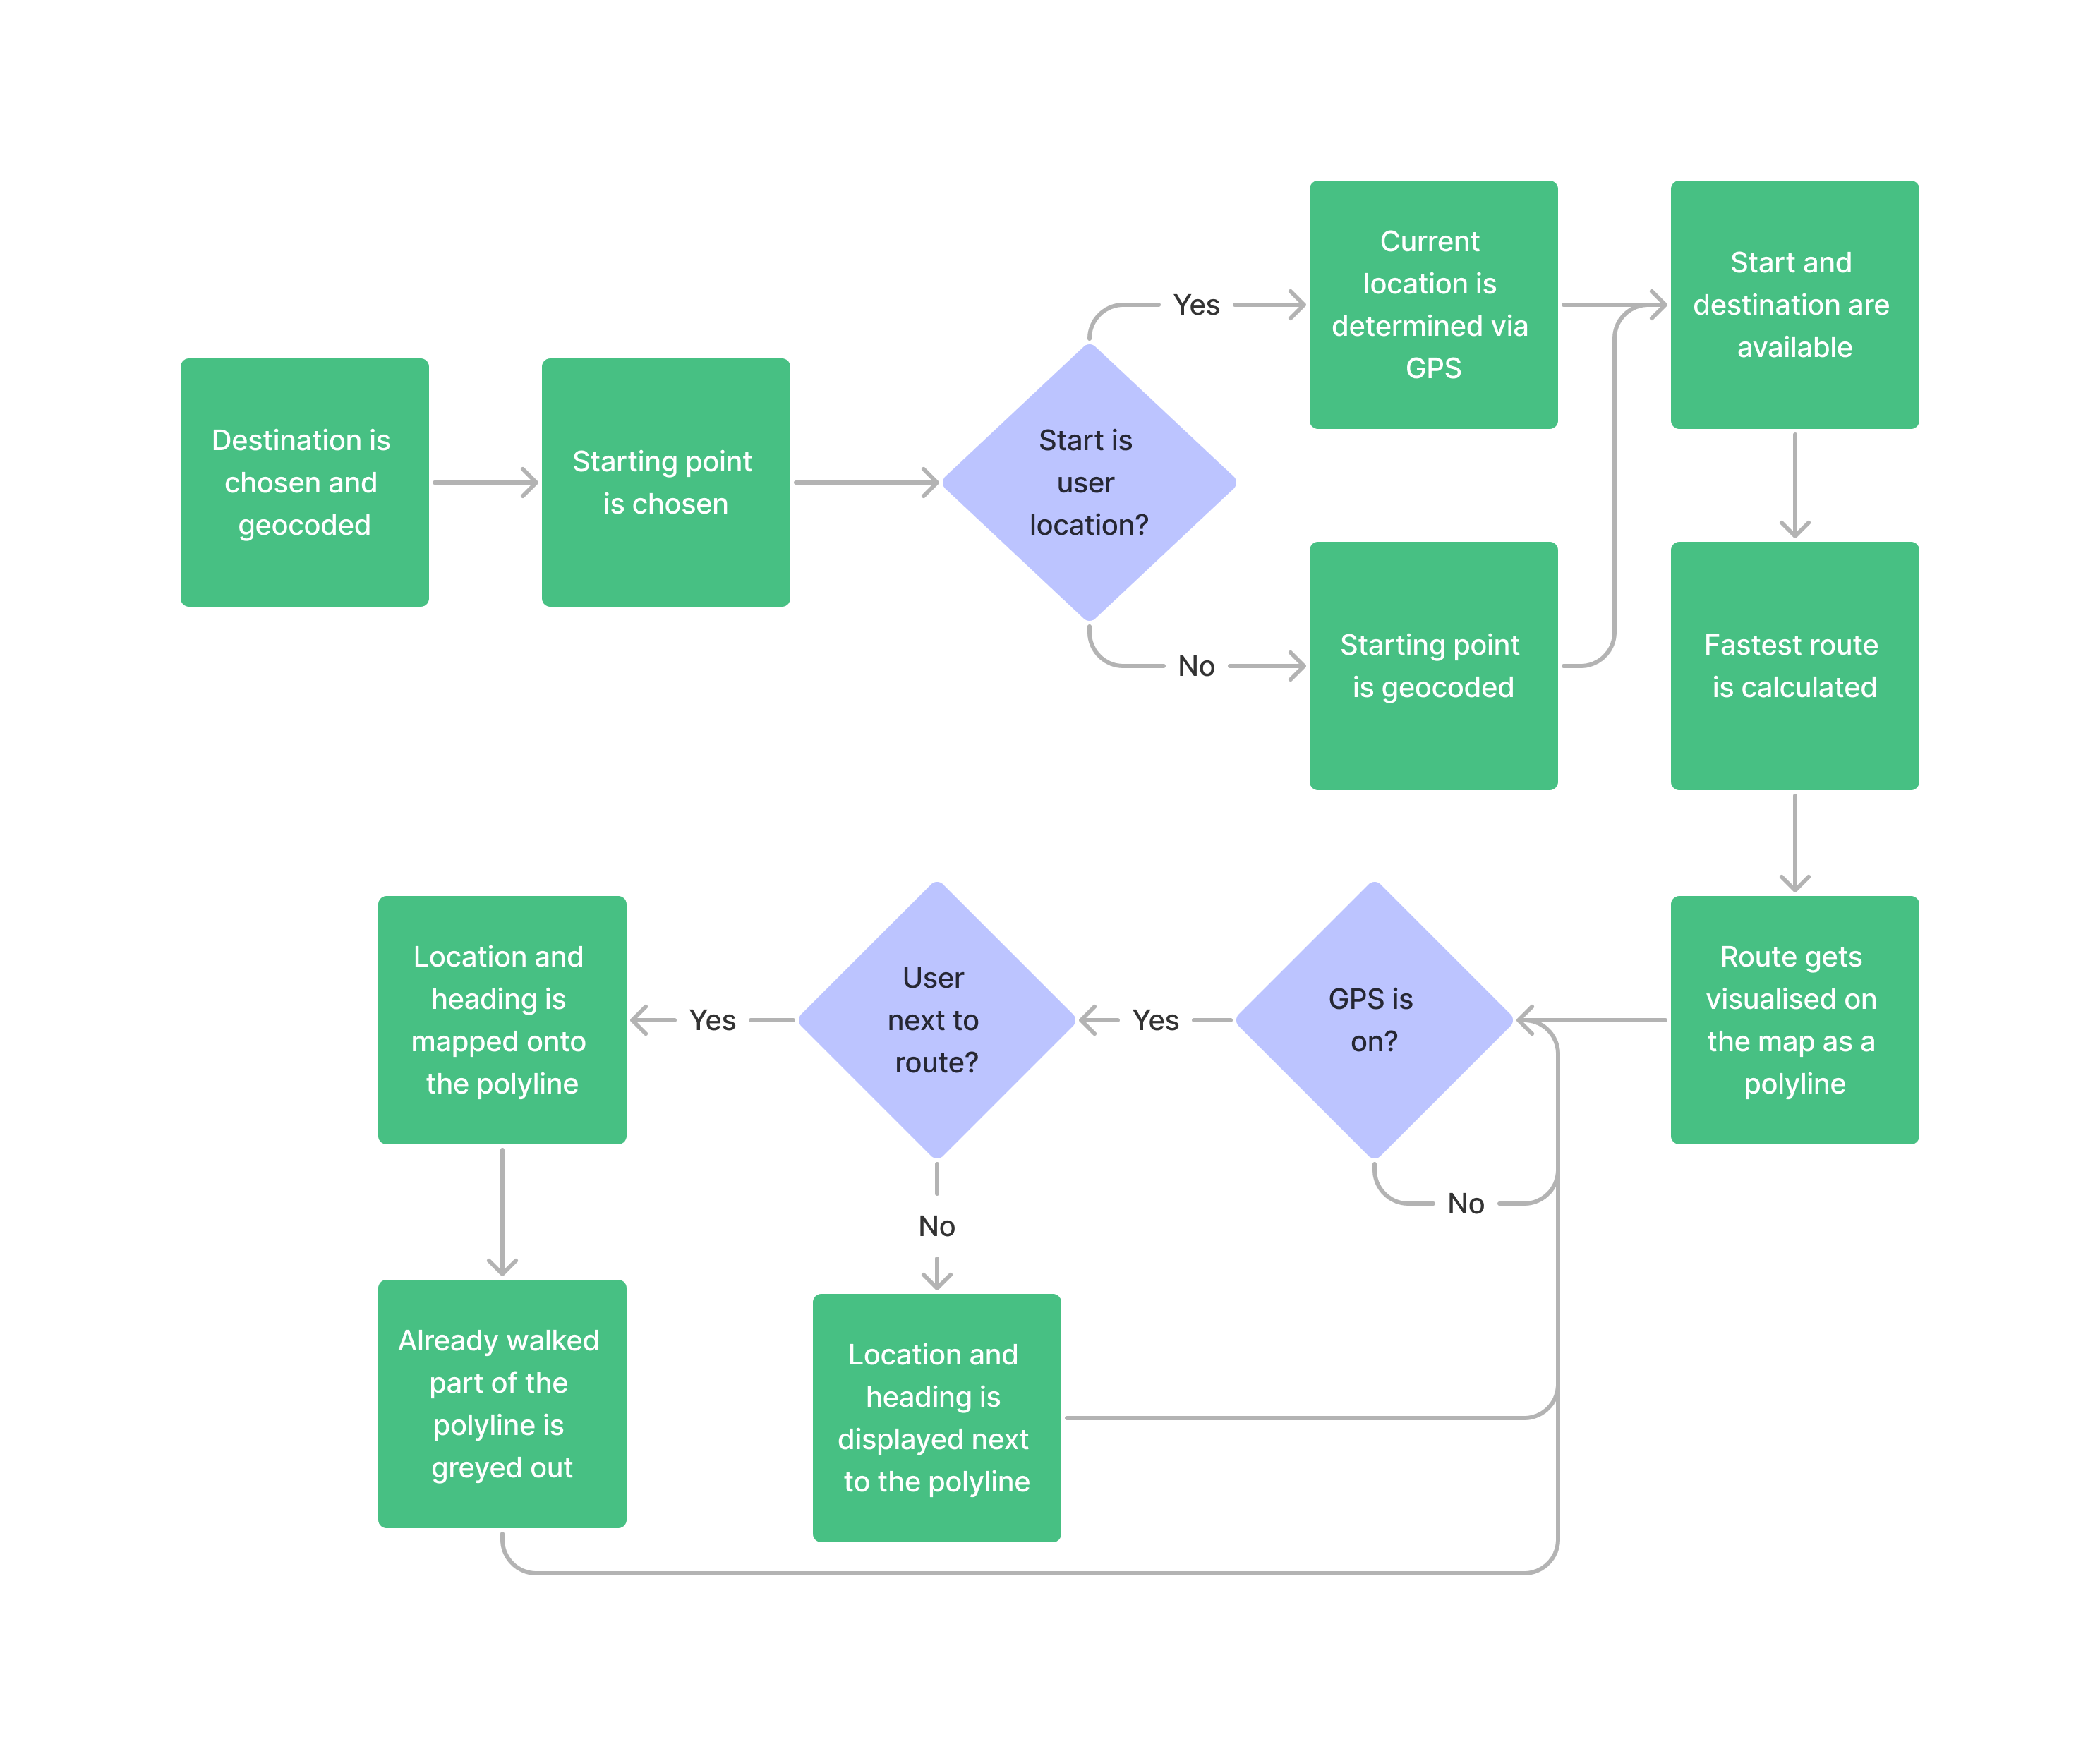
\includegraphics[width=0.85\textwidth]{images/navigation_process.png}\\
	\caption{Complete navigation system procedure}
\end{figure}

\subsection{Information layer}
An additional layer on top of the campus map consisting of location-based information is a natural addition to the feature set of the mobile app. It enhances the user experience, the relevance of the whole product and the overall digital information culture of TU Berlin by providing overlays, markers and labels filled with data about the campus.

This section provides a brief overview of the underlying data and technology used to provide the information on the layer.

There are three main sources, that are publicly available and relevant to the information layer. On the one hand, there is the official website of TU Berlin \cite{tu_berlin_main}, with sections for current events, the latest news, deadlines, etc. On the other hand, there is the MOSES system \cite{tu_berlin_moses} containing data about all the different courses, rooms and studies. A third relevant source of information is the website of Studierendenwerk Berlin \cite{studierendenwerk_berlin} with meal plans for its different canteens and a timetable for events.

Information is collected by downloading and parsing the content of respective websites. The data is further categorized and -if possible- mapped onto different POIs on the campus map (e.g., a canteen gets its meal plan assigned). This helps to provide an intuitive and organized presentation and access to the user.

The collected data can be categorized according to its timeliness and the intervals in which it has to be updated: General information about different fields of study, courses and rooms only changes by semester. This particular data can be retrieved once at the start of every semester and does not need daily live updates. It is also possible to supply it via app updates, instead of providing a direct in-app functionality for data retrieval. Data that gets updated regularly on the other hand, e.g., meal plans, events, news, etc. has to be always retrievable from the app.

The proposed solution for data collection and provision runs on a web server and consists of a web crawler for information retrieval, parsing and POI mapping, a CSV generator to convert the crawled information into a standardized and simple-to-use format and a REST API, that provides the client/mobile device the ability to retrieve the CSV files. The web crawler and CSV generator are both triggered periodically by several CRON jobs, whose timings are dependent on the timeliness of the crawled data. Due to its simplicity, the circumstance that there are no complex relations in the data and the fact that all room data from TU Berlin is provided in it, the CSV format is chosen as an alternative to a fully-fledged database system for data storage.

By splitting the logic for crawling and provision, the workload that arises on TU Berlin's and Studierendenwerk's websites from retrieving data can be limited to a minimum: The server only crawls data when an update is needed (e.g., weekly for meal plans), instead of loading and parsing the web resources on client request. Further advantages are the fact that loading times for requests from clients are independent of TU Berlin's and Studierendenwerk's infrastructure, that the language for web crawling can be chosen independently from the programming framework (in this case Python with its Selenium \cite{selenium} and BeautifulSoup \cite{beautifulsoup4} libraries are used) and that the web crawling logic can be changed without updating the app.

\begin{figure}[H]
	\centering
	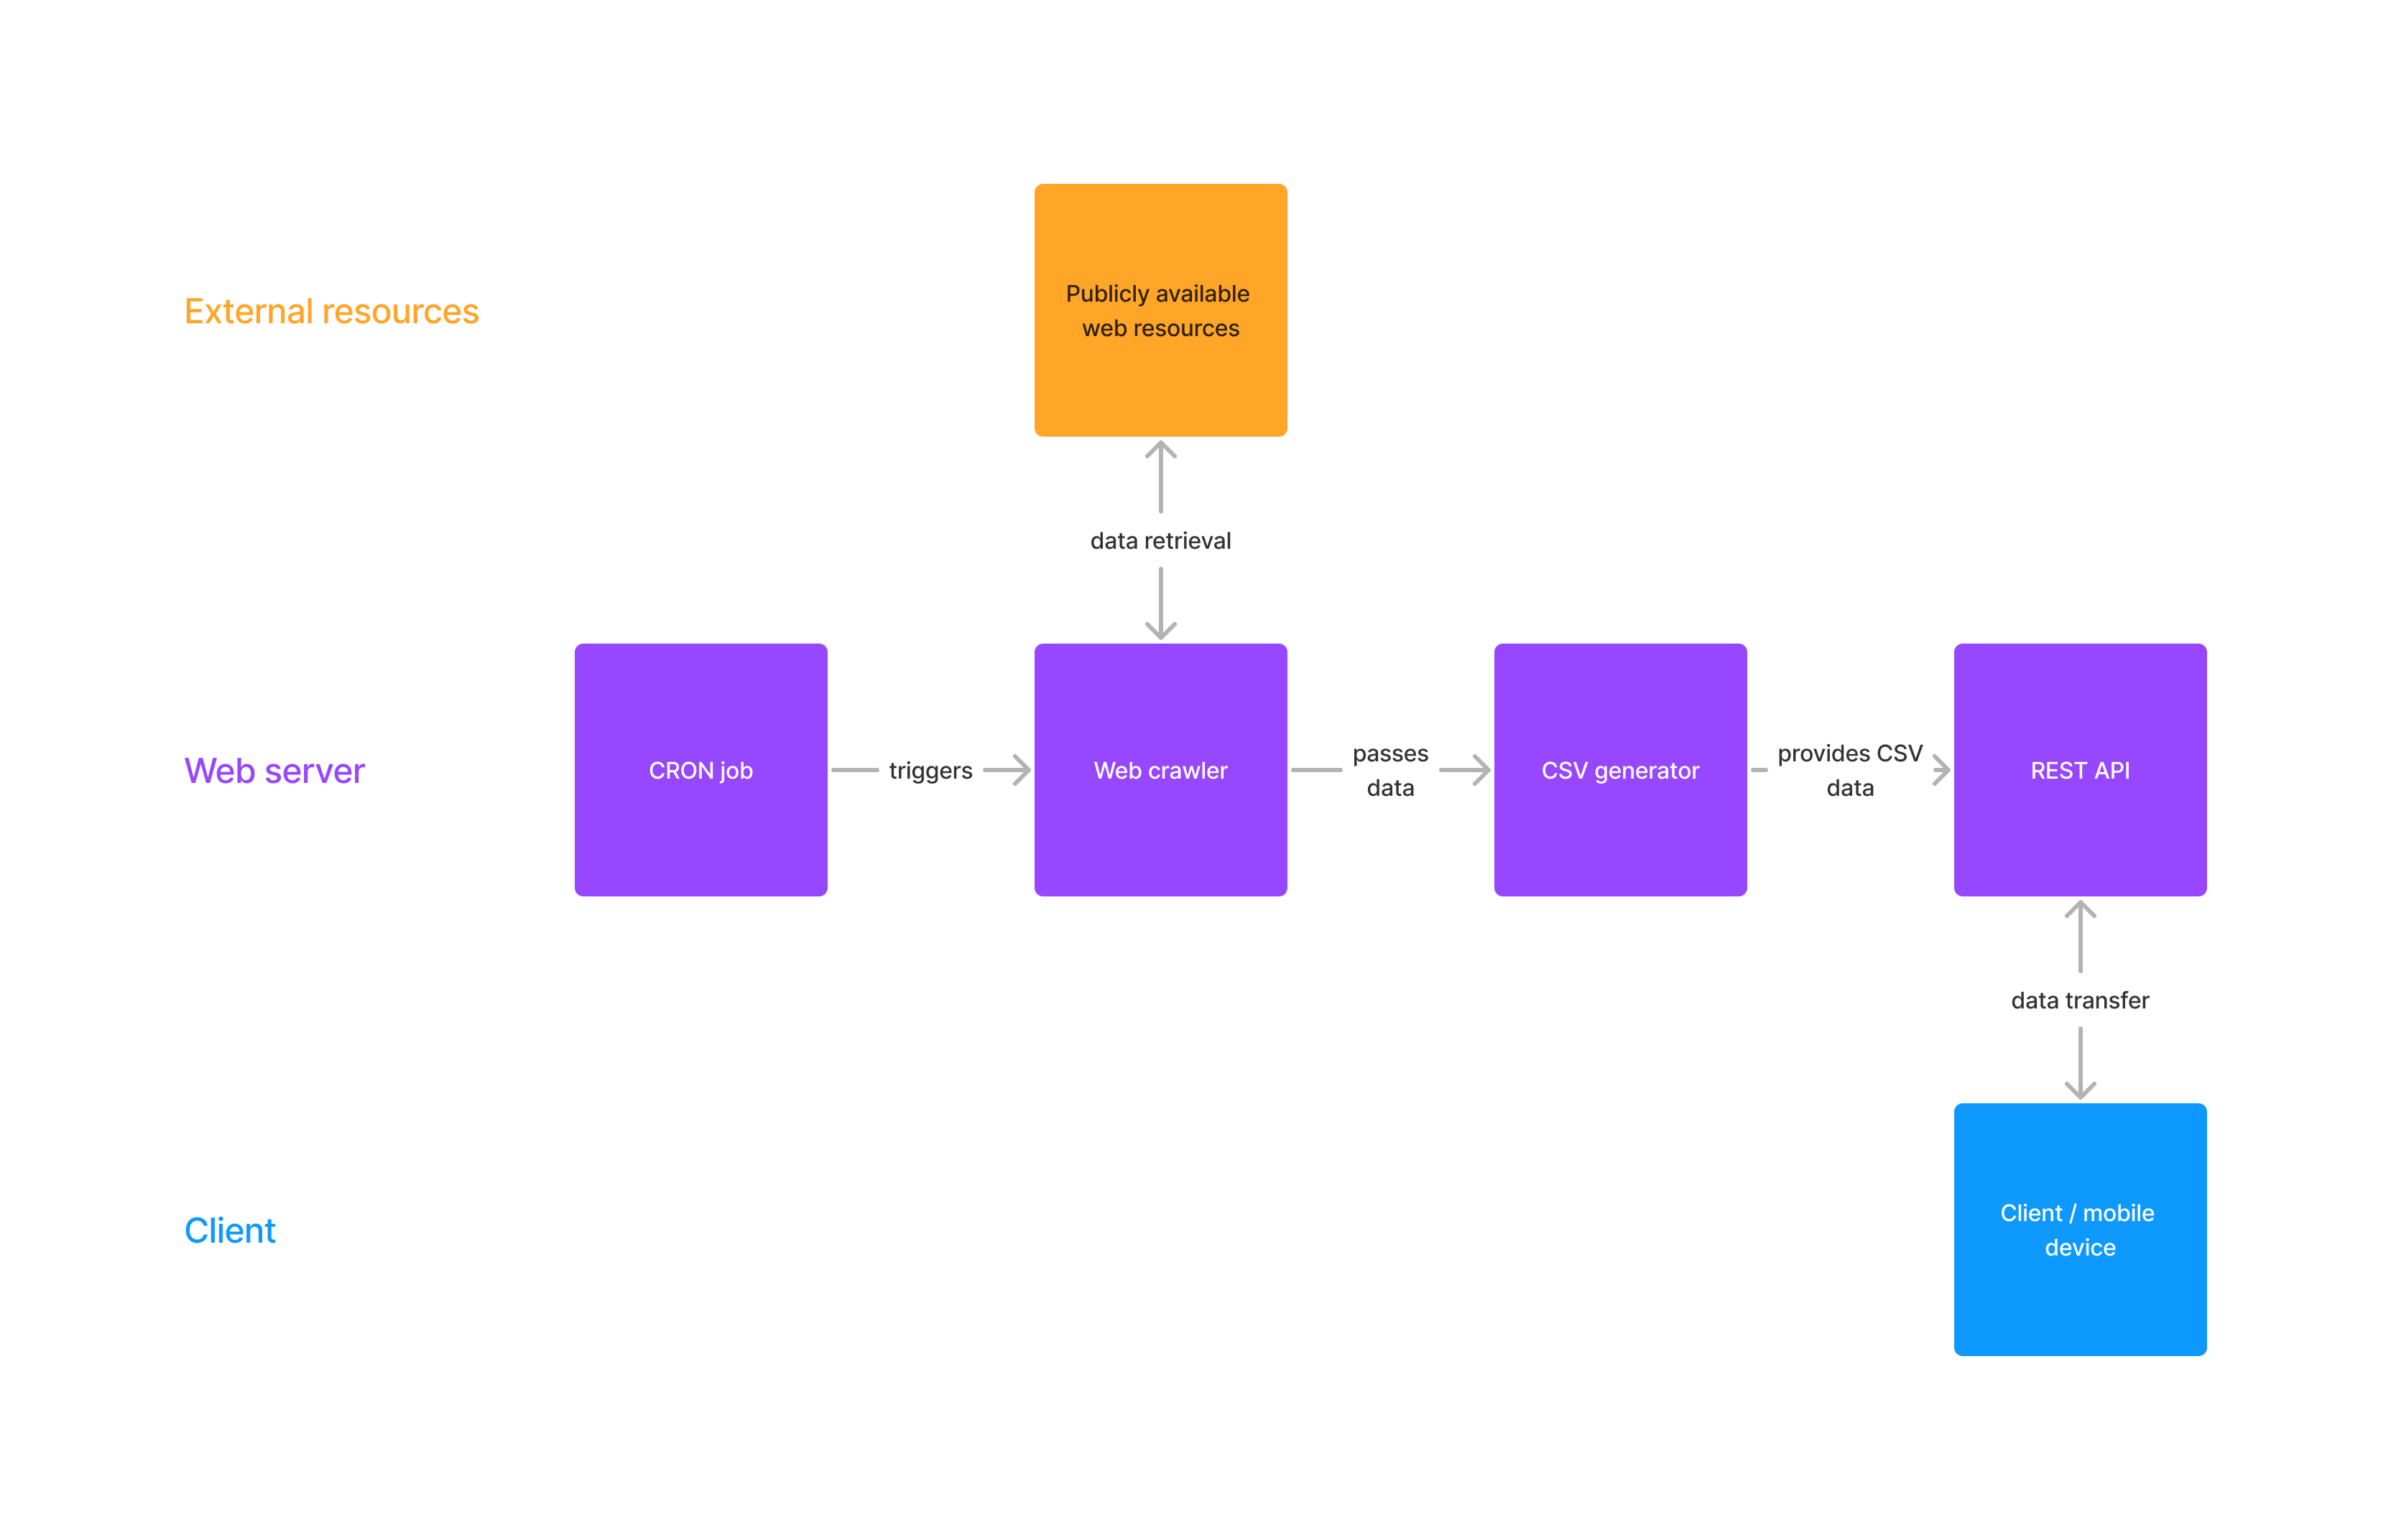
\includegraphics[width=0.85\textwidth]{images/information_layer_backend.png}\\
	\caption{Data retrieval process for the information layer}
\end{figure}

%\subsection{Exploration vs. search}
%\subsection{Search functionality}
%\subsection{Alternative presentation of information}

\subsection{Offline-first design}
One important aspect of the app concept is an extensive focus on offline usability. The whole system is designed to allow the user (as far as possible) a network-connection-free app usage. This applies in particular to the navigation system, the campus map and the information layer of the app:

Campus map: The campus map is locally implemented on the device. All necessary information can be therefore loaded and used without a network connection.

Navigation system: Due to the comparatively small scope of the navigation system, the weighted graph for navigation as well as the system for routing can both be implemented and executed on-device. Only the navigation feature working with live user location updates relies on stable GPS functionality.

Information layer: Loading and presenting information on TU Berlin's main campus requires access to the respected online resources and cannot be realized without a network connection. The need for network connectivity can be nevertheless reduced: Since no data requires real-time updates (the most critical data being meal plans that require weekly updates), the data for the information layer can be stored locally after download and loaded from memory for the remaining week. This approach reduces the need for internet connectivity to a minimum.

%This can be realized by sending silent push notifications at the start of every week. Devices that cannot receive the synchronizing push notification can download the data while being used. At best, this system allows the user to use the app throughout the week without going online.

\section{App development framework}
The choice of app development framework is an important step while conceptualizing and designing the product. It determines the programming language of the project, the built-in device- and system-specific capabilities that can be accessed during development as well as the performance of the app. It has to be selected in consideration of the project's requirements. The following enumeration presents the most important demands for this thesis:
\begin{itemize}
    \item Used technologies: Working with low-level hardware and operating system APIs is an important part of development. Technologies and systems used in the key features of the product (e.g., GPS capabilities) have to be accessible or implemented in the selected framework.
    \item Cross-platform capabilities: Native app development is complex and time-consuming. Learning and especially working with two different codebases (Java / Kotlin for Android, Swift / Obj. C for IOS) is difficult and not possible within the scope of this thesis. Cross-platform frameworks solve this problem by providing the ability to work with a single codebase for different operating systems.
    \item Focus on high-quality user interfaces: One of the most important requirements of the app development framework is the availability to easily build high-quality and modern user interfaces with it. 
    \item Execution speed: Regarding the fact that the whole navigation functionality has to take place locally on the phone, the speed with which the code of the mobile app gets executed is crucial to a responsive and fast user experience. Particularly the algorithms used for routing have to be reliably computable within seconds.
    \item 3d rendering capabilities: The framework needs to provide a way to render and interact with the created 3d model of campus Charlottenburg. Further built-in systems such as an extensive linear algebra toolkit, a lighting engine and other real-time rendering capabilities also need to be taken into account.
\end{itemize}

Based on the previously defined requirements, the Flutter framework \cite{flutter} is chosen for this work. In addition to its cross-platform capabilities, it also offers the ability to compile source code into platform-specific machine code for near-native execution performance. It further comes with access to thousands of packages through the dart package manager pub \cite{pub_dev}, an extensive set of pre-built components for user interfaces and the ability to write platform-specific code for low-level API access. Since Flutter lacks 3d rendering capabilities, the Unity engine \cite{unity_engine} is additionally used to create and display the campus map. It gets included in the Flutter build and is responsible for rendering and interacting with the 3d campus map.

\section{User experience design}
The following sections provide an overview of the whole user experience (UX) design for the campus app. In the scope of this thesis, the complete process is broken down into UX research and wireframe design.

UX research is a process where the main goals and tasks associated with the app are identified and broken down into its most relevant UX aspects. This helps to find out the key usability requirements for the visual user interface design, consisting of wireframes and high-fidelity mockups (user interface design).

Wireframes, on the other hand, form the first visual version of the app design. They determine the basic structure of the app, its layout, the placement of basic user interface elements as well as their hierarchy. Wireframes are based on the previously defined usability requirements in the UX research process.

The next paragraphs describe a set of important usability requirements that are then further incorporated into the wireframe design.

%Usability goals: Search versus exploration
\subsection{Search versus exploration}
One of the most important usability requirements for the app results from the clash of two important user needs, namely search and exploration. These needs result from the fact that users may use the app for different purposes and with different expectations.\\

Search, on the one hand, describes a scenario, in which the user tries to find or locate a specific piece of information within the app. This search for information can be expressed with concrete questions, e.g.:

\begin{itemize}
    \item What is the fastest way between MAR and TEL buildings?
    \item What are the opening times of the TU library?
    \item What food can I get tomorrow at the main cafeteria?
    \item Where does course App-Entwicklung take place?
    \item In which building is the SNET department located?
\end{itemize}

One main requirement for the user experience of the app is therefore the possibility for fast, easy and structured access to important key information about TU Berlin's campus. All search-task-related user interface elements should be easily identifiable as such, prominently positioned and accessible to the user. Additionally, to reduce the search time for the seeking person, the design should also provide multiple ways to access the most important information. Important user interface elements in this case are search bars, descriptive icons and textual hints as well as an adequately chunked information hierarchy in the whole app.\\

Exploration, on the other hand, is an app use case, in which the user "just browses around" in search of nothing particular. The seeking person either wants to learn, find out or experience something new or uses the app with an open question in mind. In this scenario, the user does not seek a specific piece of information but rather expects the app to provide the possibility, to easily navigate and view through structured content without the need for a concrete search.

Examples of goals and questions for exploration use cases can be the following:

\begin{itemize}
    \item Are there any interesting places on TU Berlin's campus that I could visit?
    \item Which cafeteria has the best food today?
    \item Are there any appealing courses, outside of the scope of my studies, that I can attend this semester?
    \item Search for upcoming events by TU Berlin or Studierendenwerk
    \item Search for learning spaces at TU Berlin
\end{itemize}

In these use cases, the outcome of the exploration action is often determined by the subjective preferences of the users. The app therefore cannot give an optimal final solution to the search but rather present a set of information, from which the user can select or find the most suitable one.

This results in two important requirements for the app design. Firstly, visual elements for the structured presentation of information need to be used. Examples of that can be tables, scrollable lists, clearly designed information cards and different kinds of markers on the campus map. These elements help the user by giving hints about existing information in the app and by structuring related information, which then can be easily overviewed and potentially compared while exploring.

Secondly, the choice of which information is portrayed in the app is important. Since too much information provision risks a bloating of the app (and therefore a reduced user experience), the final campus data needs to be carefully selected and filtered for in-app display. The establishment of a clear hierarchy between important, frequently used data and less important information also contributes to this.

\subsection{Designing a user-friendly campus map}

\subsection{Chunking of information within the app}

\section{User interface design}
\chapter{Implementation}
\label{cha:implementation}
\section{Collection of geodata and POI}
\subsection{Overview of needed geodata}
\subsection{Collection data from OSM via Overpass Turbo API}
\subsection{Enhancing OSM data with manually collected data}

\section{Generation of digital campus map}
\subsection{Merging geodata in QGIS}
\subsection{Map design}
\subsection{Offline integration within the mobile app}
\subsection{3-dimensional presentation of university buildings}

\section{Navigation system development}
\subsection{Representation of geodata for navigation}
\subsection{Routing across the campus}
\subsection{Time estimation for routes}
\subsection{Embedding the current user location via GPS}

\section{Interactive information layer development}
\subsection{Collection of campus relevant information from the web}
\subsection{Processing of information and internal representation}

\section{User interface development}
\subsection{Navigation system}
\subsection{Information layer}
\subsection{Enhancing the user experience with additional screens and features}
\chapter{Evaluation}
\label{cha:evaluation}
This section provides an overview of a set of metrics used to compare the developed campus app to the already-established navigation solutions for mobile devices (Google Maps and Apple Maps). Furthermore, all steps regarding implementation, data acquisition and measurement as well as the resulting consequences for the respective metric are presented.

\section{Campus map verfication} \label{sec:campus_map_verification}
The digital campus map of TU Berlin forms the app's most important element. It is therefore essential to evaluate and compare its implementation to other digital maps. This section presents an overview of different metrics that can be evaluated quantitatively for map verification and compares the actual measurements to the geolocation services of Android and IOS.

To verify the campus map, an important emphasis must be laid on the correctness and quality of the underlying geodata. To achieve this, two different benchmarks, one for measuring the geographical resolution of a map and one for measuring its geocoding capabilities, are introduced in the following sections.

%the map resolution of campus Charlottenburg, which indicates the level of detail on the map, as well as the geocoding capabilities of the system, %mainly the mapping of university-specific identifiers and names to their respective campus entities, are compared.

%Einmal die Abstände bei zufälligen Koordinaten und zwischen Gebäude-Koordinaten und den Eingängen messen
\subsection{Comparison of map resolution}
The geographical resolution of a map describes the level of detail that the underlying geodata has. A more detailed set of geodata can result in better map visualization for the user interface (improving usability as well as localization capabilities) and a more complex underlying navigation graph that can calculate individual routes more precisely.

To measure a comparable indicator for the geographical resolution of a particular map, the underlying geocoding API of the respective mobile app provider is used. This API provides the possibility to query the system's most fitting geodata points for a particular geographical input (pair of latitude and longitude).

It can be assumed that the distances of the candidate points returned by a geocoding API to the original point can be seen as a metric that indicates the geodata coverage of the specified region, with low distances suggesting that the system contains an adequate representation of the area around the geographic campus point. The following list describes the set of steps that are performed to measure this map resolution metric for the whole campus:

\newpage

\begin{enumerate}
    \item A random set of $N$ geographical points $P = \{p_{0}, p_{1}, p_{2}, \ldots\}$, each lying on campus Charlottenburg, is generated
    \item The set of the system's most fitting candidate points $C_{i} = \{c_{i_{0}}, c_{i_{1}}, c_{i_{2}}, \ldots\}$ is queried for each random point $p_{i}$ from the respective geocoding API
    \item The distances $D_{i} = \{dist(p_{i}, c_{i_{0}}), dist(p_{i}, c_{i_{1}}), dist(p_{i}, c_{i_{2}}), \ldots\}$ are calculated
    \item The minimal distance $d_{i} = \min(D_{i})$ for each point $p_{i}$ is retrieved and the average of all minimal distances $\frac{d_{0} + d_{1} + d_{2} + \cdots + d_{N}}{N}$ for a specific geocoding provider is calculated
    \item These averaged values are compared between geocoding engines and provide an indicator for the geographical node coverage of each system's campus representation
\end{enumerate}

\vspace{2mm}

For practical implementation, the campus is split into \hyperref[table:campus_regions]{3 bounding boxes}. A total of 250 random geographic points are generated for each bounding box and the average closest point distances are calculated for every campus region and each geocoding provider API (campus app, Android and IOS). The following figure presents the results:

\begin{figure}[H]
	\centering
	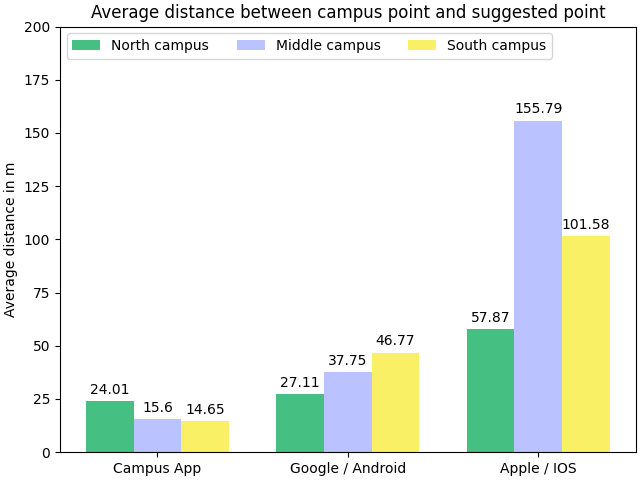
\includegraphics[width=0.75\textwidth]{images/average_campus_point_distance.png}\\
	\caption{Average distance between campus point and suggested point}
\end{figure}

The figure shows that the campus app outperforms the geocoding capabilities of the Android and IOS geocoding services on randomly sampled point datasets for every region of campus Charlottenburg by factors 1 to 3 for Google Maps and 2 to 10 for Apple Maps.

The values for the entire campus are 18,08 m for the campus app, 37,21 m (approx. factor 2) for Google Maps and 105,08 m (approx. factor 5) for Apple Maps. When extrapolated for the entirety of all geographical points on the campus, it can be concluded that the overall resolution of campus Charlottenburg differs by presented factors between those geocoding APIs.

\newpage

To provide a more differentiated evaluation of the campus coverage, a set of heatmaps is created, each displaying the map of campus Charlottenburg with the geodata coverage of the respective geocoding API.

\begin{figure}[H]
	\centering
	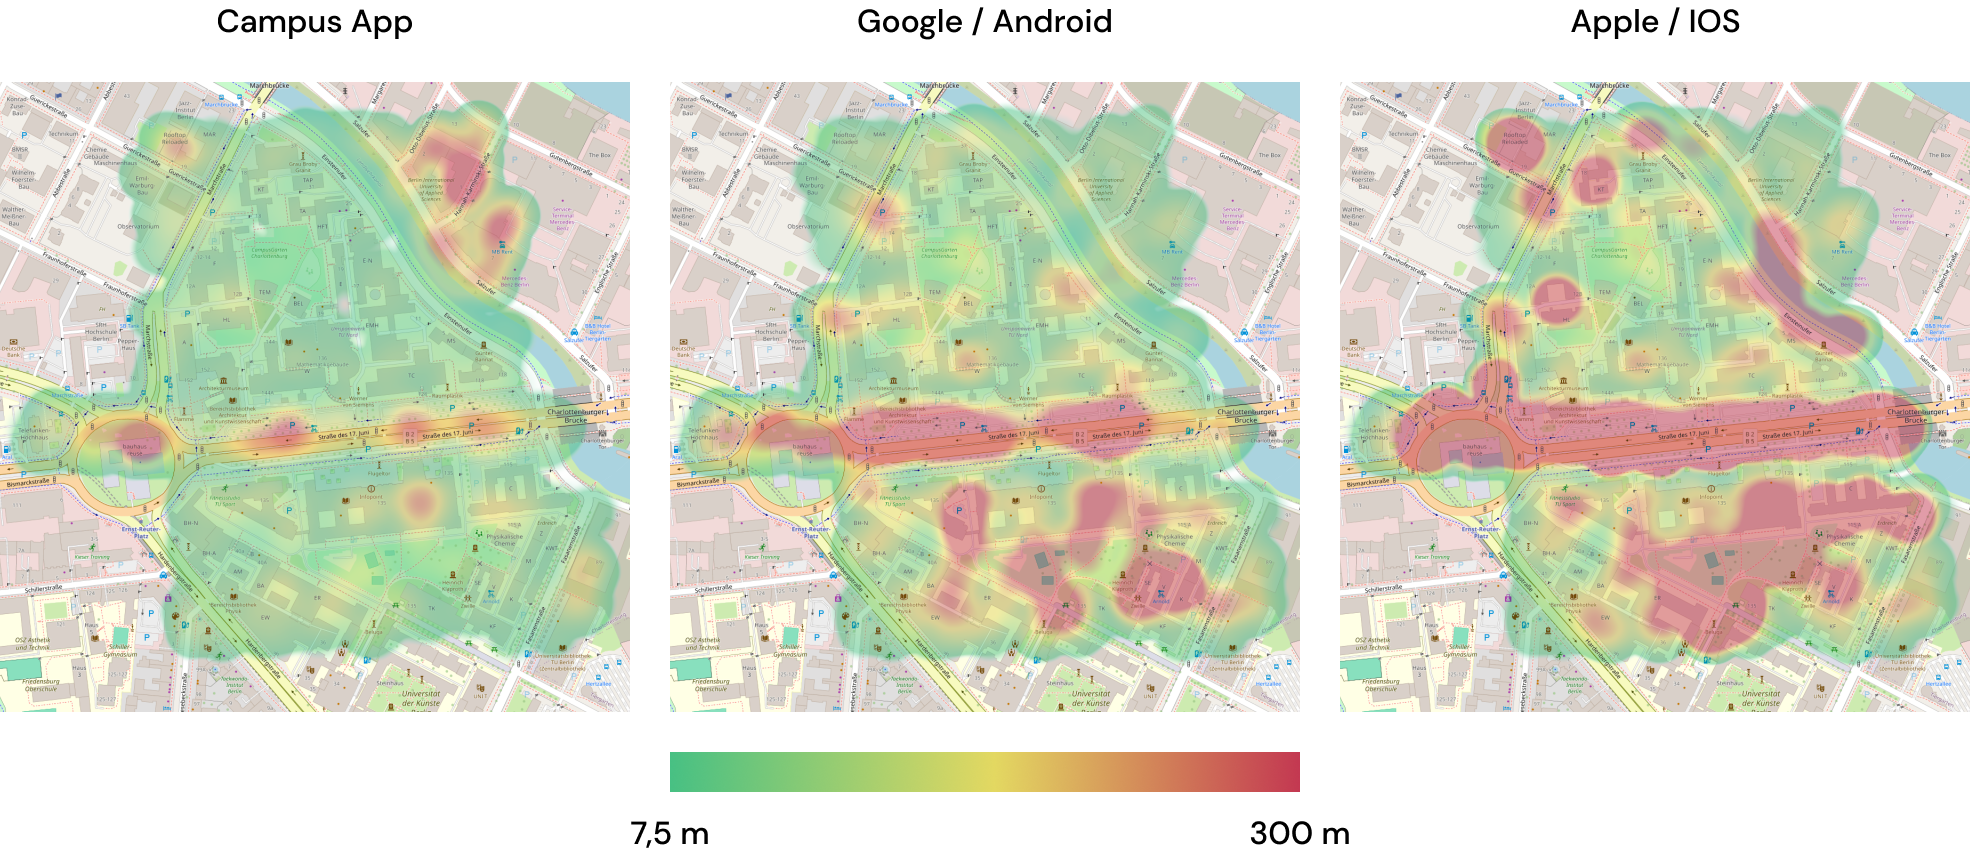
\includegraphics[width=1.0\textwidth]{images/heatmaps.png}\\
	\caption{Heatmaps for campus map coverage by average point distance}
\end{figure}

One important factor that can be seen in both data representations is the fact that the north side of campus Charlottenburg has a better geodata coverage than both other sections throughout all different providers. The heatmaps also present the fact that the campus app has the best average campus resolution and that its resolution weaknesses can (since no important entity or pathway is located in these areas) be seen as negligible for the proper functionality of the system.

Generally can be said that the Android geolocation services are more precise than the IOS counterparts in the scope of campus Charlottenburg. Both systems nevertheless struggle when points are queried for the south side of campus Charlottenburg as well as for Straße des 17. Juli. The latter weakness mostly arises from the fact that every geolocation in the campus-splitting section of Straße des 17. Juli gets mapped onto the TU main building.

\subsection{Comparison of geocoding capabilities for campus-specific names and identifiers}
One important factor for the usability of a geocoding system is the resolution of human-readable entity names and identifiers into their respective geographic coordinates. Regarding the focus on TU Berlin's campus in Charlottenburg, a system should be able to correctly identify the building's abbreviations (e.g., TEL, MAR, H, \ldots) as well as their official names (e.g., TU-Hochhaus, Marchstraße-Gebäude, Hauptgebäude, \ldots). This section provides a benchmark to measure this ability across the geocoding APIs of the campus app, Google / Android and Apple / IOS.

To perform such a benchmark, a dataset is established, containing the entirety of the campus-specific identifiers (abbreviations) and official names of TU Berlin's entities. In exceptional cases, additional commonly used building names (e.g., "Telefunken Hochhaus" instead of "TU-Hochhaus") are also added to the dataset. This dataset is then fed into the respective geocoding APIs and the sets of possible candidate points for each query are retrieved. If at least one of the resulting candidate points is located close enough to the respective center coordinates of the inputted entity (in the test case less than 100 meters away), the human-readable input is counted as recognized by the system. To compensate for the fact that the Android and IOS geocoding APIs are not focussed on TU Berlin's campus entities, the suffix "TU Berlin" is added to each query, mimicking a common user behavior when searching for campus entities in both respective mobile apps. Furthermore, the geocoding of the actual address for each building is also analyzed for reference. The following figure presents the results.

\begin{figure}[H]
	\centering
	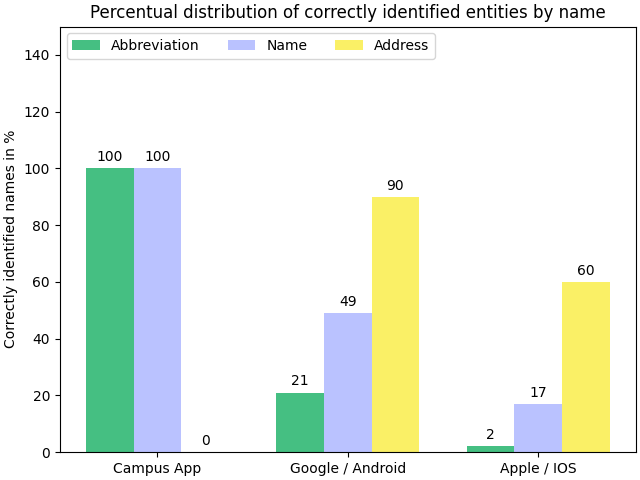
\includegraphics[width=0.75\textwidth]{images/results_geocoding_identifiers.png}\\
	\caption{Average distance between campus point and suggested point}
\end{figure}

The campus app surpasses the geocoding capabilities of Google and Apple in terms of knowledge of entity abbreviations and names. Furthermore, Google outperforms Apple throughout all categories, but both systems struggle to detect an adequate amount of abbreviations. The name metrics are in the midfield, while the systems tend to perform better when resolving direct building addresses.

\section{Navigation system verification} \label{sec:navigation_system_verification}
One important criterion for navigation system verification lies in the quality of the routes suggested by it. A route is thereby defined as the suggested path between a specified start and destination point, which, in the case of this thesis, are both part of TU Berlin's main campus in Charlottenburg. To analyze named quality for a specific route, the estimated time it takes to walk as well as its length are both measured. Lower walking times, as well as shorter route lengths, are thereby both regarded as preferable.

To perform a comparison between different navigation systems, a set of predefined start and destination points is established. The route calculation process of each navigation system is then applied to the defined reference points and the route metrics of the suggested routes are collected respectively. The navigation systems can be then compared for a specific pair of start and destination points as well as for the average metrics of the whole dataset. 

The pool of reference points for this comparison is chosen from the underlying building data of TU Berlin. Each center point of a building is added to the set and can be used as a starting and destination point for route calculation. The navigation systems therefore calculate all possible routes between TU Berlin's buildings. This comes with two advantages: On the one hand, the chosen pool of possible routes is large enough to be quantitatively meaningful. On the other hand, the navigation between different buildings portrays a common task for the target audience of the campus app and therefore mimics the expected user behavior. The chosen pool of reference points is furthermore representative of the geographical structure of campus Charlottenburg.

The following table presents the average results for the entire reference point dataset measured respectively on the campus app, Google Maps and Apple Maps.

\begin{table}[H]
	\small
	\centering
	\begin{tabular}{|l|l|l|}
		\hline
		\textbf{Navigation system}      & \textbf{Average walking time}       & \textbf{Average route length}  \\
		\hline
        Campus App             & 6 min 44 s	              	& approx. 510 m         \\
		\hline
        Google Maps            & 9 min 30 s              	& approx. 690 m         \\
		\hline
		Apple Maps             & 9 min 38 s              	& approx. 670 m         \\
		\hline
	\end{tabular}
	\caption{Comparison of walking time and route length}
\end{table}

The measured key figures suggest average time savings of 30\% (Google Maps) and 30\% (Apple Maps) as well as average distance savings of 23\% (Google Maps) and 20\% (Apple Maps) when the route recommended by the campus app is chosen over its counterparts. To further analyze the underlying factors for this speedup, the percentual route metrics are split according to the underlying route length suggested by the campus app:

\begin{figure}[H]
	\centering
	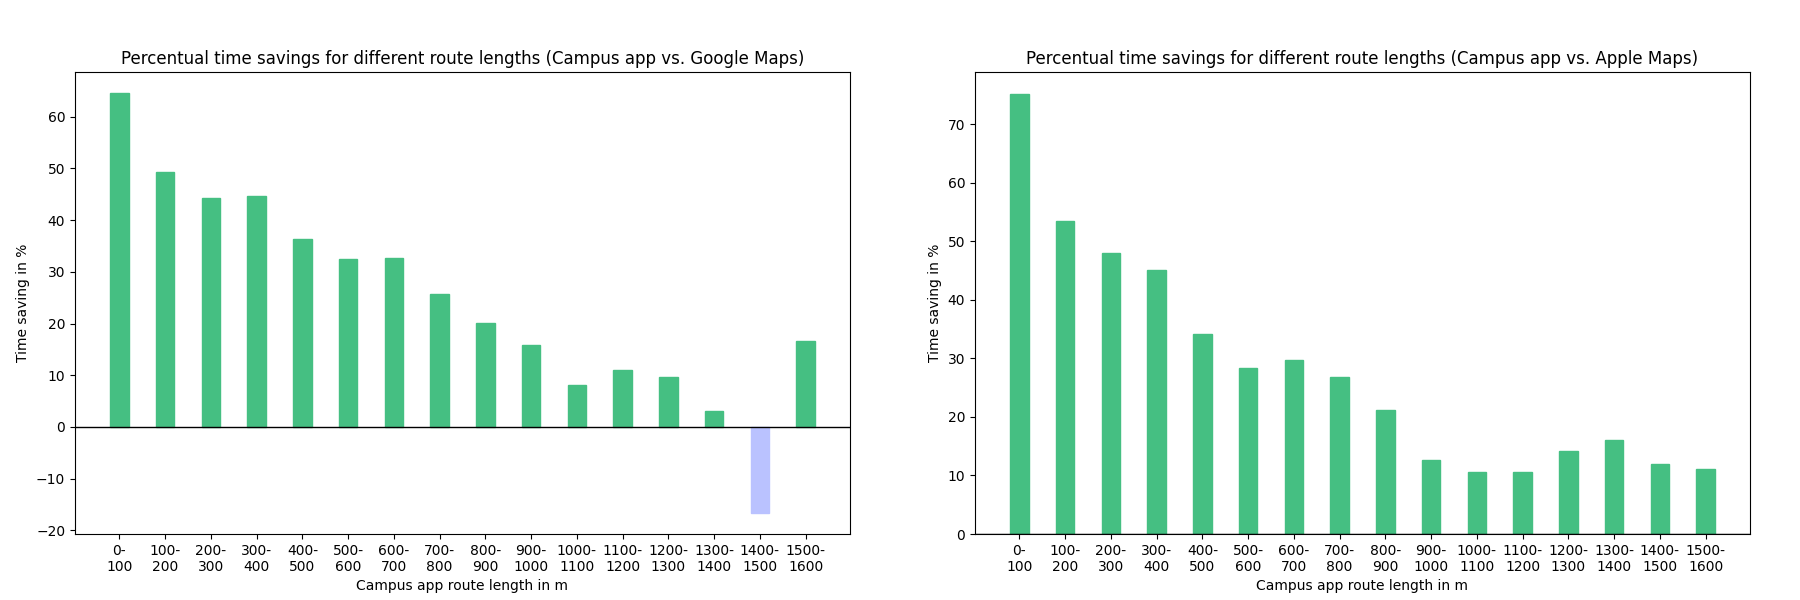
\includegraphics[width=1.0\textwidth]{images/time_differences.png}\\
	\caption{Average percentual time savings for different route lengths}
\end{figure}

\begin{figure}[H]
	\centering
	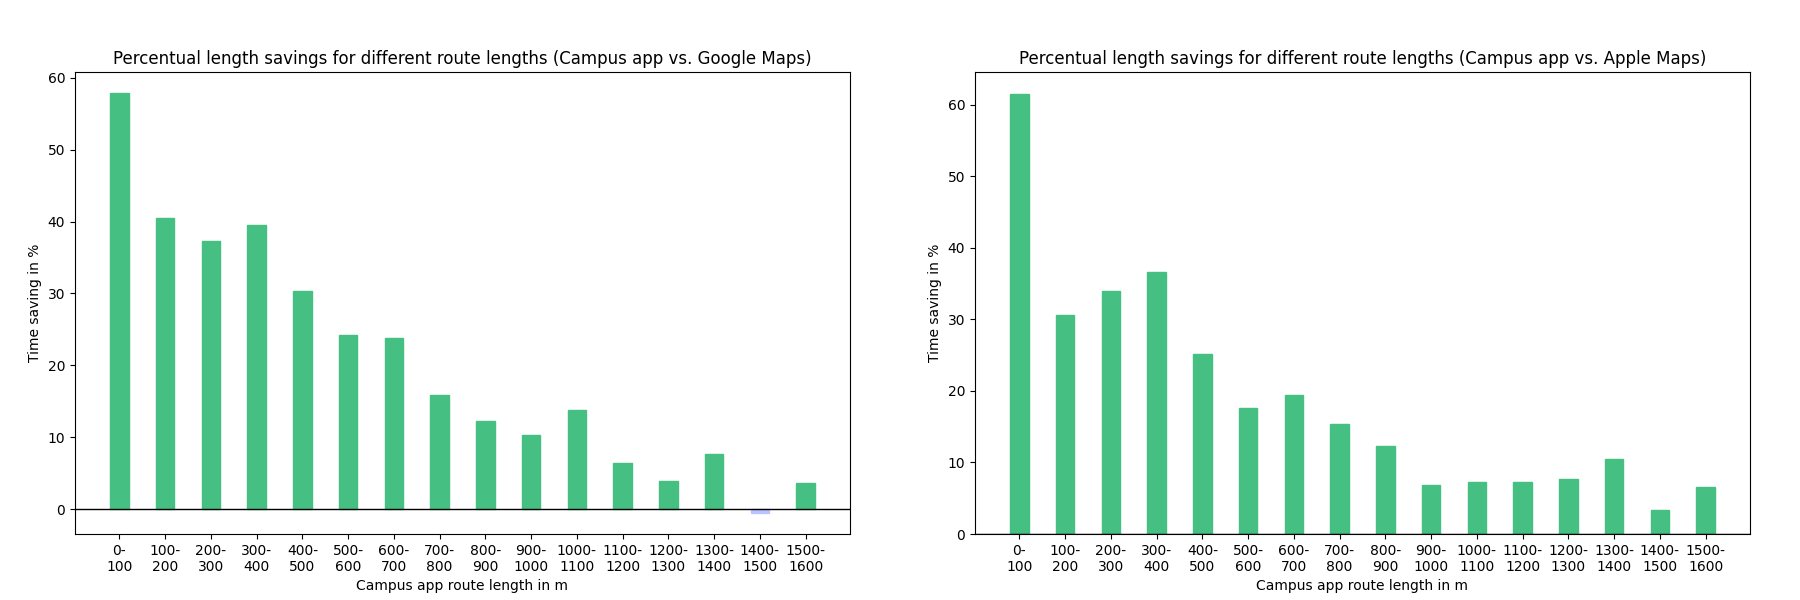
\includegraphics[width=1.0\textwidth]{images/length_differences.png}\\
	\caption{Average percentual distance savings for different route lengths}
\end{figure}

One main evaluation point that can be derived from the plots is the fact that through all route length categories (except for the distance interval of 1.4 km to 1.5 km in the Google Maps comparison), the suggested routes from the campus app always result in faster and shorter paths. This speedup is especially high for shorter routes (< 700 m) and declines with increasing route length. The overall biggest speedup is achieved in the category for routes under 100 meters. In this section, start and destination points often lay in different but connected buildings. The routing for this circumstance can be solved very efficiently by the campus app as an indoor route between both buildings can be proposed.

% \section{Information layer verification}

\chapter{Conclusion}
\label{cha:conclusion}

%--------------------------------------------------------------
% TABLES, FIGURES, BIBLIOGRAPHY AND APPENDICES
%--------------------------------------------------------------
\backmatter

% Lists of tables and figures
\listoftables
\listoffigures

% Bibliography
\setwidesite{}						% Set page to be wider for bibliography
\markboth{Bibliography}{bibliography}
\label{cha:bibliography}
\bibliographystyle{IEEEtran}
\bibliography{bibliography.bib}

% Use the following to separate online (websites) and offline (books, papers) sources
%\printbibliography[heading=offline,filter=offline]
%\printbibliography[heading=online,filter=online]

\begin{appendices}
	\chapter{Appendix 1}
\label{appendix:listing1}

\lstset{language=SQL}
\begin{lstlisting}[caption={Overpass Turbo query for all of TU Berlin's buildings}, label={buildings}]
[bbox:52.49993096650543, 13.307022255971093, 52.52269751545147, 13.341918533901309];
(
        way["building"="university"];>;
        way(456211792);>;
        way(358373103);>;
        way(104507902);>;
        way(290166587);>;
        way(172802144);>;
        way(262367508);>;
        way(48793247);>;
        way(50557514);>;
        way(993968604);>;
        way(993968602);>;
);
out meta;
\end{lstlisting}

\begin{lstlisting}[caption={Overpass Turbo query for all main roads next to the campus}, label={main_roads}]
[bbox:52.49993096650543, 13.307022255971093, 52.52269751545147, 13.341918533901309];
(
    way["highway"="primary"];>;
    way["highway"="secondary"];>;
);
out meta;
\end{lstlisting}

\begin{lstlisting}[caption={Overpass Turbo query for all small roads next to the campus}, label={small_roads}]
[bbox:52.49993096650543, 13.307022255971093, 52.52269751545147, 13.341918533901309];
(
    way["highway"="residential"];>;
    way["highway"="tertiary"];>;
);
out meta;
\end{lstlisting}

\begin{lstlisting}[caption={Overpass Turbo query for all pathways and sidewalks next to the campus}, label={pathways}]
[bbox:52.49993096650543, 13.307022255971093, 52.52269751545147, 13.341918533901309];
(
    way["highway"]["highway"!="primary"]["highway"!="secondary"]["highway"!="residential"]["highway"!="tertiary"][!"footway"];>;
);
out meta;
\end{lstlisting}

\begin{lstlisting}[caption={Overpass Turbo query for all water green next to the campus}, label={green_areas}]
[bbox:52.49993096650543, 13.307022255971093, 52.52269751545147, 13.341918533901309];
(
    way["landuse"="grass"];>; 
    way["leisure"="park"];>;
    way["leisure"="garden"];>; 
    way["natural"="scrub"];>; 
    way(314528756);>; 
    way(104712588);>;
    way(531886237);>;
    way(531886252);>;
);
out meta;
\end{lstlisting}

\begin{lstlisting}[caption={Overpass Turbo query for water areas next to the campus}, label={water}]
[bbox:52.49993096650543, 13.307022255971093, 52.52269751545147, 13.341918533901309];
(
    way["natural"="water"];>;
);
out meta;
\end{lstlisting}

\begin{lstlisting}[caption={Overpass Turbo query for all entrances to buildings on the campus}, label={entrances}]
[bbox:52.49993096650543, 13.307022255971093, 52.52269751545147, 13.341918533901309];
node["entrance"];
out meta;
\end{lstlisting}

\begin{table}[H]
    \small
    \centering
    \begin{tabular}{|l|l|l|}
        \hline
        Region name              & North-West coordinates                           & South-East coordinates  \\
        \hline
        North Campus             & (52.51667973620, 13.32222127479)	              	& (52.5133200241, 13.329653624217)        \\
        \hline
        Middle Campus            & (52.513220529803, 13.319945039190)              	& (52.5127460156, 13.330647119317)         \\
        \hline
        South Campus             & (52.512386299901, 13.323101586912)              	& (52.51048052265, 13.33127591368)         \\
        \hline
    \end{tabular}
    \caption{Different campus regions}
    \label{table:campus_regions}
\end{table}

	\chapter{List of abbreviations}
\label{appendix:abbreviations}

\vspace*{25px}
\begin{tabular}{lp{5cm}}
    \textbf{Abbreviation}               &               \textbf{Definition} \\
    POI                                 &               Point of interest \\
    OSM                                 &               OpenStreetMap \\
    PDR                                 &               Pedestrian dead reckoning \\
    ETA                                 &               Estimated time of arrival \\
    Obj. C                              &               Objective C \\
    UX                                  &               User experience \\
    UI                                  &               User interface \\
    HEX                                 &               Hexadecimal \\
    UVs                                 &               UV coordinates \\
    FOV                                 &               Field of view \\
\end{tabular}
	% \input{content/99_appendices/a03_listings}
\end{appendices}

\end{document}
